%% LyX 2.3.6.2 created this file.  For more info, see http://www.lyx.org/.
%% Do not edit unless you really know what you are doing.
\documentclass[twocolumn,conference]{IEEEtran}
\usepackage[T1]{fontenc}
\usepackage[latin9]{inputenc}
\usepackage{color}
\usepackage{booktabs}
\usepackage{textcomp}
\usepackage{amsmath}
\usepackage{amssymb}
\usepackage{stmaryrd}
\usepackage{graphicx}
\usepackage[unicode=true,
 bookmarks=true,bookmarksnumbered=true,bookmarksopen=true,bookmarksopenlevel=1,
 breaklinks=false,pdfborder={0 0 0},pdfborderstyle={},backref=false,colorlinks=false]
 {hyperref}
\hypersetup{pdftitle={Your Title},
 pdfauthor={Your Name},
 pdfpagelayout=OneColumn, pdfnewwindow=true, pdfstartview=XYZ, plainpages=false}

\makeatletter

%%%%%%%%%%%%%%%%%%%%%%%%%%%%%% LyX specific LaTeX commands.
%% Because html converters don't know tabularnewline
\providecommand{\tabularnewline}{\\}

%%%%%%%%%%%%%%%%%%%%%%%%%%%%%% Textclass specific LaTeX commands.
\newenvironment{lyxcode}
	{\par\begin{list}{}{
		\setlength{\rightmargin}{\leftmargin}
		\setlength{\listparindent}{0pt}% needed for AMS classes
		\raggedright
		\setlength{\itemsep}{0pt}
		\setlength{\parsep}{0pt}
		\normalfont\ttfamily}%
	 \item[]}
	{\end{list}}

%%%%%%%%%%%%%%%%%%%%%%%%%%%%%% User specified LaTeX commands.
% for subfigures/subtables
\usepackage[caption=false,font=footnotesize]{subfig}
\usepackage{hyperref}
\hypersetup{colorlinks=true}
\usepackage[dvipsnames]{xcolor}
\definecolor{lgray}{rgb}{0.95, 0.95, 0.95}
\usepackage{mathtools}
\usepackage{supertabular,booktabs}
\usepackage{longtable}

\@ifundefined{showcaptionsetup}{}{%
 \PassOptionsToPackage{caption=false}{subfig}}
\usepackage{subfig}
\makeatother

\usepackage[frozencache,cachedir=_minted-bragghls]{minted}
\usepackage[style=numeric,backend=bibtex]{biblatex}
\renewcommand{\listingscaption}{Listing}

\newif\iffinal
% Un-comment this line to see proposal without comments
%\finaltrue

\iffinal
  \newcommand\maxx[1]{}
  \newcommand\ian[1]{}
  \newcommand\ryan[1]{}
  \newcommand\kyle[1]{}
  \newcommand\kaz[1]{}
  \newcommand\arham[1]{}
\else
  \newcommand\maxx[1]{{\color{red}[Max: #1]}}
  \newcommand\ian[1]{{\color{blue}[Ian: #1]}}
  \newcommand\ryan[1]{{\color{magenta}[Ryan: #1]}}
  \newcommand\kyle[1]{{\color{yellow}[Kyle: #1]}}
  \newcommand\kaz[1]{{\color{purple}[Kaz: #1]}}
  \newcommand\arham[1]{{\color{green}[Arham: #1]}}
\fi

\addbibresource{ref.bib}
\begin{document}
\title{\texttt{BraggHLS}}
\author{\IEEEauthorblockN{Maksim~Levental\\
and Arham~Khan}\IEEEauthorblockA{University of Chicago\\
Email: test@test.tes}\and \IEEEauthorblockN{Ryan~Chard\\
and Kazutomo~Yoshi}\IEEEauthorblockA{Argonne National Laboratory\\
Nantes, France\\
Email: second@second.fr}\and \IEEEauthorblockN{Kyle~Chard\\
and Ian~Foster}\IEEEauthorblockA{Star Academy\\
San Francisco, California 99999-9999\\
Telephone: (800) 555\textendash 5555\\
Fax: (888) 555\textendash 5555}}

\maketitle
\renewcommand{\MintedPygmentize}{/Users/mlevental/dev_projects/hls_paper/scripts/pygmentize.py}
\usemintedstyle{colorful}
\definecolor{bg}{rgb}{0.95,0.95,0.95}
\setminted{
    bgcolor=bg,
    escapeinside={||},
    mathescape=true,
}
\setmintedinline{breaklines}
\AtBeginEnvironment{minted}{%
  \catcode`?\active
  \begingroup\lccode`~=`\?\lowercase{\endgroup\def~{\linebreak}}%
}
\DeclareRobustCommand{\perc}{{%
  \mbox{%
    \fontencoding{\encodingdefault}%
    \fontfamily{pcr}%
    \selectfont
    \symbol{`\%}%
  }%
}}
\begin{abstract}
In many experiment-driven scientific domains, such as high-energy
physics, material science, and cosmology, very high data rate experiments
impose hard constraints on the corresponding data acquisition systems:
collected data must either be indiscriminately stored for post-processing
and analysis, thereby necessitating large storage capacity, or accurately
filtered in real-time, thereby necessitating low latency processing.
Deep neural networks, effective in many other filtering tasks, have
not been widely employed in such data acquisition systems, due to
design and deployment difficulties. This paper presents an open source,
lightweight, compiler framework \texttt{BraggHLS}, based on high-level
synthesis techniques, for translating high-level representations of
deep neural networks to low-level representations, suitable for deployment
to near-sensor devices such as field-programmable gate arrays. We
evaluate \texttt{BraggHLS} on various workloads and present a case-study
implementation of a deep neural network for Bragg peak detection in
the context of high-energy diffraction microscopy. We show \texttt{BraggHLS}
is able to produce an implementation of the network with a throughput
4.8 \textmu s/sample, which is approximately a 4$\times$ improvement
over the existing implementation.

\tableofcontents{}
\end{abstract}


\section{Introduction\label{sec:Introduction}}

Very high data rates are observed and, consequently, large datasets
are generated across a broad range of experiments in scientific domains,
such as high-energy physics, material science, and cosmology. For
example, in high-energy physics, the LHCb detector, at the CERN Large
Hadron Collider, is tasked with observing the trajectories of particles
produced in proton-proton collisions at a rate of 40 million per second
(i.e., 40 MHz)~\cite{pmlr-v42-glig14}. With a packet size of approximately
50 kB (per collision), this implies a data rate of approximately 2
TB/s. Ultimately, in combination with other detectors, the LHC processes
approximately 100 EB of data per year. In materials science, high-energy
diffraction microscopy (HEDM) techniques, which provide non-destructive
characterization of structure and its evolution in a broad class of
single-crystal and polycrystalline materials, can have collection
rates approaching 1 MHz~\cite{Hammer_2021}, with a corresponding
packet size of 80 kB. In cosmology, the Square Kilometer Array, a
radio telescope projected to be completed in 2024 and to be operational
by 2027~\cite{mcmullin2022square}, will sustain data rates in excess
of 10 TB/s~\cite{grainge2017square}.

Naturally, for high data rate experiments, directly storing and distributing
such large quantities of data to the associated research communities
for further analysis is cost prohibitive. Thus, either compression
(in the case of storage and transmission) or outright filtering is
necessary, i.e., only a small fraction of the most ``interesting''
data is selected at time of collection, with the remainder being permanently
discarded. In this work we focus on the filtering approach. Note,
the tradeoff made in employing filtering should be clear: reduced
storage at the expense of more stringent latency constraints (on the
filtering mechanisms). Typically, these filtering mechanisms consist
either of physics based models~\cite{LHCB-FIGURE-2020-018} or machine
learning models~\cite{Gligorov_2013}; in either case maximally efficient
and effective use of the target hardware platform is important. Irrespective
of the type of technique employed, almost universally, for the ultra-low
latency use cases (e.g., sub-microsecond latency constraints), the
implementation is deployed to either field-programmable gate arrays
(FPGAs) or application-specific integrated circuits (ASICs)~\cite{Duarte_2018}.
Here we focus primarily on FPGAs.

Deep neural networks (DNNs), a particular type of machine learning
model, have been shown to be effective in many scientific and commercial
domains due to their ``representational capacity'', i.e., they demonstrate
a capacity to (approximately) represent diverse sets of mappings~\cite{alzubaidi2021review}.
DNNs ``learn'' to represent a mapping over the course of ``training'',
wherein they are iteratively evaluated on sample data while a ``learning
rule'' periodically updates the \emph{weights} that parameterize
the DNN. In recent years they have been investigated for near real-time
scientific use cases~\cite{liu2019deep,patton2018167,liu2022exploring}
but their use for the lowest latency use cases has been limited~\cite{Duarte_2018}.
The reasons for this are threefold:
\begin{enumerate}
\item Graphics Processing Units (GPUs), the conventional hardware target
for DNNs, until very recently, have not been performant enough for
these very high data rate, very low latency, use cases (due to their
low clock speeds and low peripheral bandwidth~\cite{aaij2020allen});
\item DNNs, by virtue of their depth, are resource intensive, in terms of
both memory (for the weights) and compute (floating-point arithmetic),
thereby preventing their deployment to FPGAs, which, in particular,
have limited static RAM available;
\item DNNs are (typically) defined, trained, and distributed using high-level
frameworks (such as PyTorch~\cite{paszke2017automatic}, TensorFlow
\cite{https://doi.org/10.48550/arxiv.1603.04467}, MXNet~\cite{https://doi.org/10.48550/arxiv.1512.01274}),
which abstract all implementation details from the user, thereby making
portability of existing model architectures (to e.g., FPGA) nigh impossible.
\end{enumerate}
These three barriers demand of a solution that can simultaneously
translate a high-level representation of a DNN to a low-level representation,
suitable for deployment to FPGA, while optimizing resource usage and
minimizing latency. In general, the task of \emph{lowering} high-level
representations of programs to low-level representations is the domain
of a compiler. Similarly, the task of \emph{synthesizing} a\emph{
register-transfer level} (RTL) \emph{design}, rendered in a \emph{hardware
description language} (HDL), from a program, is the domain of high-level
synthesis (HLS)~\cite{7368920} tools. While several such HLS tools
exist~\cite{10.1145/2514740,Zhang2008,ferrandi2021bambu} they struggle
to effectively perform the necessary optimizations in reasonable amounts
of time (see Section~\ref{subsec:High-level-synthesis}) despite,
often, bundling robust optimizing compilers,.

Recently, deep learning compilers (such as TVM~\cite{chen2018tvm},
MLIR~\cite{https://doi.org/10.48550/arxiv.2002.11054}, and Glow~\cite{https://doi.org/10.48550/arxiv.1805.00907})
have demonstrated the ability to dramatically reduce inference latencies
\cite{https://doi.org/10.48550/arxiv.1809.02697}, training times
\cite{9664259}, and memory usage~\cite{https://doi.org/10.48550/arxiv.1604.06174}
of DNNs. These compilers function by extracting intermediate-level
representations (IRs) of the DNNs, from the representations produced
by the frameworks, and performing various optimizations on those IRs
(such as kernel fusion~\cite{10.1145/2858788.2688521}, vectorization
\cite{maleki2011evaluation}, and memory planning~\cite{https://doi.org/10.48550/arxiv.1604.06174}).
The highly optimized IR is then used to generate code for various
target hardware platforms. Given the successes of these compilers,
it's natural to wonder whether they can be adapted to the task of
sufficiently optimizing a DNN such that it might be synthesized to
RTL, for deployment to FPGA.

In this paper, we present \texttt{BraggHLS}, an open source, lightweight,
compiler and HLS framework which can lower DNNs defined as PyTorch
models to FPGA compatible implementations. \texttt{BraggHLS} uses
a combination of compiler and HLS techniques to compile the entire
DNN into fully scheduled RTL, thereby eliminating all synchronization
overheads and achieving low latency. \texttt{BraggHLS} is general
and supports a wide range of DNN layer types, and thus a wide range
of DNNs, but we particularly focus on optimizations relevant to a
DNN designed for identifying Bragg diffraction peaks. In summary our
specific contributions include:
\begin{enumerate}
\item We describe and implement a compiler framework, \texttt{BraggHLS},
which can effectively transform unoptimized, hardware-agnostic PyTorch
models into low latency RTL designs suitable for deployment to Xilinx
FPGAs. \texttt{BraggHLS} is thoroughly tested, open source, and available
at \href{https://github.com/makslevental/bragghls/}{https://github.com/makslevental/bragghls/};
\item We show that designs generated by \texttt{BraggHLS} achieve lower
latency than Xilinx's state-of-the-art commercial HLS tool (Vitis
HLS) for a variety of DNN layer types. In particular we show that
\texttt{BraggHLS} can produce synthesizable designs that meet placement,
routing, and timing constraints for \texttt{BraggNN}, a DNN designed
for identifying Bragg diffraction peaks;
\item We discuss some of the challenges faced even after successful synthesis
of RTL from a high-level representation of a DNN, namely during the
place and route phases of implementation.
\end{enumerate}
The rest of this paper is organized as follows: Section~\ref{sec:Background}
reviews key concepts from compilers, high-level synthesis, and RTL
design for FPGA. Section~\ref{sec:BraggHLS-compiler-and} describes
the \texttt{BraggHLS} compiler and HLS framework in detail. Section
\ref{sec:Evaluation} evaluates \texttt{BraggHLS}\textquoteright s
performance, scalability, and competitiveness with designs generated
by Vitis HLS. Section~\ref{sec:BraggNN-case-study} describes our
case study, i.e., \texttt{BraggHLS} applied to \texttt{BraggNN}, a
Bragg peak detection DNN with a target latency of 1 \textmu s/sample.
Finally, Section~\ref{sec:Conclusion} concludes with a summary, and
related and future work.

\section{Background\label{sec:Background}}

\subsection{Compilers: the path from high to low}

The path from a high-level, abstract, representation of a DNN to a
register-transfer level representation can be formulated as a series
of progressive lowerings between adjacent levels of abstraction. Each
level of abstraction is rendered as a programming language, IR, or
HDL, and thus we describe each lowering in terms the representations
and tools \texttt{BraggHLS} employ in manipulating those representations:
\begin{enumerate}
\item An imperative, \emph{define-by-run,} Python representation, in PyTorch;
\item High-level data-flow graph representation, in TorchScript;
\item Low-level data and control flow graph representation, in MLIR.
\end{enumerate}
%

\subsubsection{PyTorch and TorchScript}

Typically DNN models are represented in terms of high-level frameworks,
themselves implemented within general purpose programming languages.
Such frameworks are popular because of their ease of use and large
library of example implementations of various DNN model architectures.
\texttt{BraggHLS} targets the PyTorch framework, thus we focus on
relevant aspects of PyTorch. DNNs developed within PyTorch are \emph{defined-by-run}:
the author imperatively describes the DNN in terms of high-level operations,
using python, which, when executed, materializes the (partial) high-level
data-flow graph (DFG) corresponding to the DNN (e.g., for the purposes
of reverse-mode automatic differentiation). From the perspective of
the user, define-by-run enables fast iteration at development time,
possibly at the cost of some runtime performance.

On the other hand, from the perspective of compilation, define-by-run
precludes efficient extraction of the high-level DFG; since the DFG
is materialized only at runtime, it cannot easily be inferred from
the textual representation (i.e., the python source) of the DNN. Furthermore,
a priori, the runtime-materialized DFG is only partially materialized\footnote{``...instead, every intermediate result records only the subset of
the computation graph that was relevant to their computation.''~\cite{paszke2017automatic}}, and only as an in-memory data structure. Thus, framework support
is necessary for efficiently extracting the full DFG. Indeed, PyTorch
supports a Single Static Assignment (SSA) IR, called TorchScript (TS)
IR and accompanying tracing mechanism (the TS JIT), which generates
TS IR from conventionally defined PyTorch models. Lowering from PyTorch
to TS IR enables various useful analyses and transformations on a
DNN at the level of the high-level DFG but targeting FPGAs requires
a broader collection of transformations. To this end, we turn to a
recent addition to the compiler ecosystem.

\subsubsection{MLIR\label{subsec:MLIR}}

Multi-level Intermediate Representation~\cite{https://doi.org/10.48550/arxiv.2002.11054}
presents a new approach to building reusable and extensible compiler
infrastructure. MLIR is composed of a set of \emph{dialect} IRs, subsets
of which are mutually compatible, either directly or by way of translation/legalization.
The various dialects aim to capture and formalize the semantics of
compute intensive programs at varying levels of abstraction, as well
as namespace related sets of IR transformations. The entrypoint into
this compiler framework, from PyTorch, is the \texttt{torch} dialect
\cite{torch-mlir}, a high-fidelity mapping from TS IR to MLIR native
IR, which, in addition to performing the translation to MLIR, fully
refines all shapes of intermediate tensors in the DNN (i.e., computes
concrete values for all dimensions of each tensor); this is necessary
for downstream optimizations and eliminating inconsistencies in the
DNN~\cite{https://doi.org/10.48550/arxiv.2203.08402}.

While the \texttt{torch} dialect is necessary for lowering to MLIR
and shape refinement, it is a representation of a DNN at the same
level of abstraction as TS IR: it does not capture the precise data
flow and control flow necessary for de novo implementations of DNN
operations (e.g., for FPGA). Fortunately, MLIR supports lower-level
dialects, such as the \texttt{linalg}, \texttt{affine} and \texttt{scf}
dialects. The \texttt{scf} (structured control flow) dialect describes
standard control flow primitives, such as conditionals and loops,
and is mutually compatible with the \texttt{arith} (arithmetic operations)
and \texttt{memref} (memory buffers) dialects. The \texttt{affine}
dialect, on the other hand, provides a formalization of semantics
that lend themselves to polyhedral compilation techniques~\cite{polyhedral-mlir},
i.e., techniques that enable loop dependence analysis and loop transformations.
Such loop transformations, particularly loop unrolling, are crucial
for achieving lowest possible latencies~\cite{yehpca2022scalehls}
because loop nests directly inform the concurrency and parallelism
of the final RTL design.

\subsection{High-level synthesis and FPGA design}

\subsubsection{High-level synthesis\label{subsec:High-level-synthesis}}

High-level synthesis tools produce RTL descriptions of designs from
high-level representations, such as C or C++~\cite{10.1145/2514740,ferrandi2021bambu}.
In particular, Xilinx's Vitis HLS, based on the Autopilot project
\cite{Zhang2008}, is a state-of-the-art HLS tool. Given a high-level,
procedural, representation, HLS carries out three fundamental tasks,
in order to produce a corresponding RTL design:
\begin{enumerate}
\item HLS schedules operations (such as \texttt{mulf}, \texttt{addf}, \texttt{load},
\texttt{store}) in order to determine which operations should occur
during each clock cycle; such a schedule depends on three characteristics
of the high-level representation:
\begin{enumerate}
\item The topological ordering of the DFG/CFG of the procedural representation
(i.e., the dependencies of operations on results of other operations
and resources);
\item The delay for each operation;
\item The user's desired clock rate/frequency;
\end{enumerate}
\item HLS associates (called \emph{binding}) floating point operations to
RTL instantiations of intellectual property (IP) for those operations;
for example whether to associate an addition operation followed by
a multiply operation to IPs for each, or whether to associate them
both with a single IP, designed to perform a ``fused'' multiply-accumulate
(MAC);
\begin{enumerate}
\item In the case of floating-point arithmetic operations, HLS also (with
user guidance) determines the precision of the floating-point representation;
\end{enumerate}
\item HLS builds a finite-state machine (FSM) that implements the schedule
of operations as control logic, i.e., logic that initiates operations
during the appropriate stages of the schedule.
\end{enumerate}
In addition to fulfilling these three fundamental tasks, high-level
synthesis aims to optimize the program. In particular, HLS attempts
to maximize concurrency and parallelism (number of concurrent operations
scheduled during a clock-cycle) in order maximize the throughput and
minimize the latency of the final implementation. Maximizing concurrency
entails pipelining operations: operations are executed such that they
overlap in time when possible, subject to available resources. Maximizing
parallelism entails partitioning the DNN into subsets of operation
that can be computed independently and simultaneously and whose results
are aggregated upon completion.

While HLS aims to automatically optimize various characteristics of
a design, there are challenges associated with this kind of automated
optimization. In particular, maximum concurrency and parallelism necessitates
data-flow analysis in order to identify data dependencies amongst
operations, both for scheduling and identifying potential data hazards.
Such data-flow analysis is expensive and grows (in runtime) as better
performance is pursued. This can be understood in terms of loop-nest
representations of DNN operations; for example consider the convolution
in Listing~\ref{lis:Single-filter-convolution}.
\begin{listing}
\begin{minted}[fontsize={\footnotesize},escapeinside={||},mathescape=true]{python}
def conv2d(
  input: MemRef(|$b$|, |$c_{in}$|, |$h$|, |$w$|),
  output: MemRef(|$b$|, |$c_{out}$|, |$h$|, |$w$|),
  weight: MemRef(|$c_{out}$|, |$c_{in}$|, |$k$|, |$k$|)
):
  for i1 in range(0, |$b$|):
    for i2 in range(0, |$c_{out}$|):
      for i3 in range(0, |$h$|):
        for i4 in range(0, |$w$|):
          for i5 in range(0, |$c_{in}$|):
            for i6 in range(0, |$k$|):
              for i7 in range(0, |$k$|):
                _3 = i3 + i6
                _4 = i4 + i7
                _5 = input[i1, i5, _3, _4]
                _6 = weight[i2, i5, i6, i7]
                _7 = output[i1, i2, i3, i4]
                _8 = _5 * _6
                _9 = _7 + _8
                output[i1, i2, i3, i4] = _9
\end{minted}
\caption{Python representation of a padding $\left\lfloor k/2\right\rfloor $,
stride 1, $c_{out}$ filter convolution with $k\times k$ kernel applied
to ($\ensuremath{b},\ensuremath{c_{in}},\ensuremath{h},\ensuremath{w}$)-dimensional\texttt{
input} tensor, where $b$ is the batch size, $c_{in}$ is the number
of channels, and ($h,w$) are the height and width, respectively.\label{lis:Single-filter-convolution}}
\end{listing}
 A schedule that parallelizes (some of) the arithmetic operations
for this loop nest can be computed by first unrolling the loops up
to some ``trip-count'' and then computing the topological sort of
the operations. Using this scheduling algorithm (known as \emph{list
scheduling}), the degree to which the loops are unrolled determines
how many arithmetic operations can be scheduled in parallel. The issue
is that the \texttt{store}s and \texttt{load}s on the \texttt{output}
array prevent reconstruction of explicit relationships between the
inputs and outputs of the arithmetic operations across loop iterations.
The conventional resolution to this loss of information is to perform
\emph{store-load forwarding}: pairs of \texttt{store} and \texttt{load}
operations on the same memory address are eliminated, with the operand
of the \texttt{store} forwarded to the uses of the \texttt{load} (see
Listing~\ref{lis:Single-filter-convolution-1}).
\begin{listing}
\begin{minted}[numbers=left,fontsize={\footnotesize},escapeinside={||},mathescape=true,highlightlines={19,25},autogobble=true,numbersep=3pt]{python}
def conv2d(
  input: MemRef(|$b$|, |$c_{in}$|, |$h$|, |$w$|),
  output: MemRef(|$b$|, |$c_{out}$|, |$h$|, |$w$|),
  weight: MemRef(|$c_{out}$|, |$c_{in}$|, |$k$|, |$k$|)
):
  for i1 in range(0, |$b$|):
    for i2 in range(0, |$c_{out}$|):
      for i3 in range(0, |$h$|):
        for i4 in range(0, |$w$|):
	  ...
	  # e.g., i5, i6, i7 = 2, 3, ${\setlength{\fboxsep}{1pt}\colorbox{Salmon}{\texttt{4}}}$
	  _31 = i3 + i6
	  _41 = i4 + i7
	  _51 = input[i1, i5, _31, _41]
	  _61 = weight[i2, i5, i6, i7]
	  _71 = output[i1, i2, i3, i4]
	  _81 = _51 * _61
	  |${\setlength{\fboxsep}{1pt} \colorbox{green}{\texttt{\_91}}}$| = _71 + _81
          |${\setlength{\fboxsep}{1pt}          \colorbox{green}{\texttt{output[i1, i2, i3, i4]}}}$| = |${\setlength{ \fboxsep}{1pt} \colorbox{green}{\texttt{\_91}}}$|
	  # i5, i6, i7 = 2, 3, ${\setlength{\fboxsep}{1pt}\colorbox{Salmon}{\texttt{5}}}$
	  _32 = i3 + i6
	  _42 = i4 + i7
	  _52 = input[i1, i5, _32, _42]
	  _62 = weight[i2, i5, i6, i7]
	  |${\setlength{\fboxsep}{1pt}\colorbox{yellow}{\texttt{\_72}}}$| = |${\setlength{\fboxsep}{1pt}          \colorbox{green}{\texttt{output[i1, i2, i3, i4]}}}$|
	  _82 = _52 * _62
	  |${\setlength{\fboxsep}{1pt}\colorbox{Cyan}{\texttt{\_92}}}$| = |${\setlength{\fboxsep}{1pt}\colorbox{yellow}{\texttt{\_72}}}$| + _82
	  output[i1, i2, i3, i4] = _92
	  ...
\end{minted}
\caption{Store-load forwarding across successive iterations (e.g.,\texttt{
i7} $={\setlength{\fboxsep}{1pt}\colorbox{Salmon}{\texttt{4}}}, {\setlength{\fboxsep}{1pt}\colorbox{Salmon}{\texttt{5}}}$)
of the inner loop in Listing~\ref{lis:Single-filter-convolution},
after unrolling. The forwarding opportunity is from the store on line
19 to the load on line 25; both can be eliminated and ${\setlength{\fboxsep}{1pt}\colorbox{green}{\texttt{\_91}}}$
can replace uses of ${\setlength{\fboxsep}{1pt}\colorbox{yellow}{\texttt{\_72}}}$,
such as in the computation of \texttt{${\setlength{\fboxsep}{1pt}\colorbox{Cyan}{\texttt{\_92}}}$}
(and potentially many others).\label{lis:Single-filter-convolution-1}}
\end{listing}
 In order for this transformation to be correct (i.e., preserve program
semantics), for each pair of candidate \texttt{store} and \texttt{load}
operations, it must be verified that there are no intervening memory
operations on the same memory address. These verifications are non-trivial
since the iteration spaces of the loops need not be regular; in general
it might involve solving a small constraint satisfaction program~\cite{rajopadhye2002dependence}.
Furthermore, the number of such verifications grows polynomially in
the parameters of the convolution since the loop nest unrolls into
$b\times c_{out}\times h\times w\times c_{in}\times k^{2}$ \texttt{store}-\texttt{load}
pairs on the \texttt{output} array.

Finally, note, though greedy solutions to the scheduling problem solved
by HLS are possible, in principle, the scheduling problem is formulated
as an integer linear program (ILP), instances of which are NP-hard.
In summary, HLS tools solve computationally intensive problems in
order to produce a RTL description of a high-level representation
of a DNN. These phases of the HLS process incur ``development time''
costs (i.e., runtime of the tools) and impose practical limitations
on the amount of design space exploration (for the purpose of achieving
latency goals) which can be performed. \texttt{BraggHLS} addresses
these issues by enabling the user to employ heuristics during both
the parallelization and scheduling phases which, while not guaranteed
to be correct (but can be \emph{behaviorally verified}) and have much
lower runtimes (see Section~\ref{subsec:Symbolic-execution-for}).

\subsection{FPGA design}

Broadly, at the register-transfer level of abstraction, there remain
two more steps prior to being able to actually deploy a design to
an FPGA; one of them being a final lowering, so-called logic synthesis,
and the other being place and route (P\&R). The entire process is
carried out, for example, by Xilinx's Vivado tool.

Logic synthesis is the process of mapping RTL to actual hardware primitives
on the FPGA (so-called \emph{technology mapping}), such as lookup
tables (LUTs), block RAMs (BRAMs), flip-flops (FFs), and digital signal
processors (DSPs). Logic synthesis produces a network list (\emph{netlist})
describing the logical connectivity of various parts of the design.
Logic synthesis, for example, determines the implementation of floating-point
operations in terms of DSPs; depending on user parameters and other
design features, DSP resource consumption for floating-point multiplication
and addition can differ greatly. Logic synthesis also determines the
number of LUTs and DSPs that a high-level representation of a DNN
corresponds to, which is relevant to both the performance and feasibility
of that DNN when deployed to FPGA.

After the netlist has been produced, the entire design undergoes P\&R.
The goal of P\&R is to determine which configurable logic block within
an FPGA should implement each of the units of logic required by the
digital design. P\&R algorithms need to minimize distances between
related units of functionality (in order to minimize wire delay),
balance wire density across the entire fabric of the FPGA (in order
to reduce route congestion), and maximize the clock speed of the design
(a function of both wire delay, logic complexity, and route congestion).
The final, routed design, can then be deployed to the FPGA by producing
a proprietary \emph{bitstream}, which configures the FPGA.

\section{\texttt{BraggHLS} compiler and HLS framework\label{sec:BraggHLS-compiler-and}}

\texttt{BraggHLS} is a compiler and HLS framework which employs MLIR
for extracting loop-nest representations of DNNs. It is implemented
in python for ease of use and extensibility. Critically, and distinctly,
it handles the DNN transformations as well as scheduling, binding,
and FSM extraction; there is no dependence on any commercial HLS tools.
Figure~\ref{fig:BraggHLS-framework-overview.-3} shows the architecture
of \texttt{BraggHLS}
\begin{figure}[tbh]
\centering{}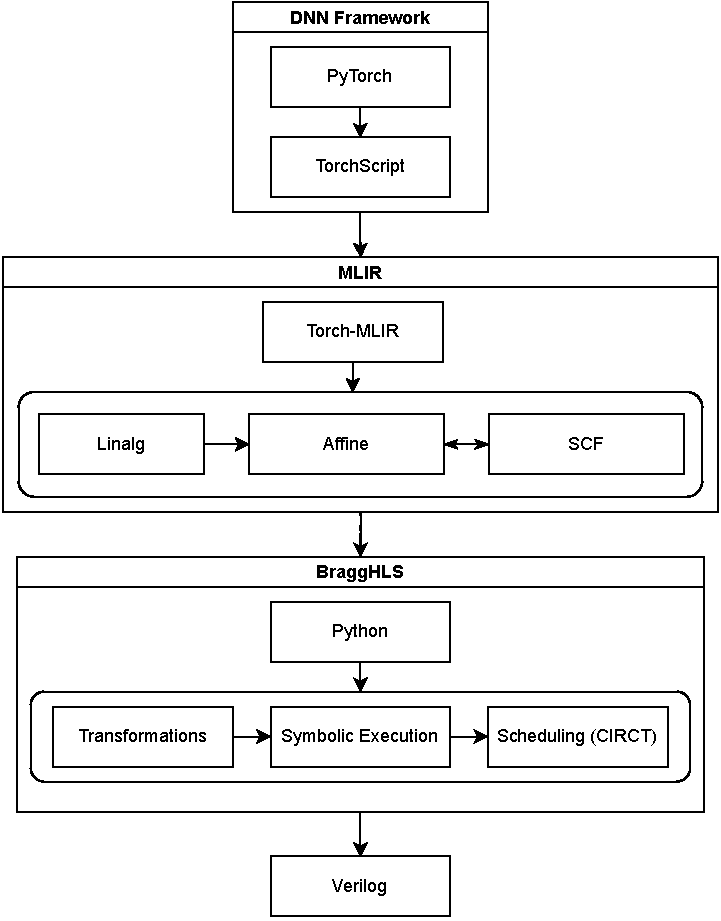
\includegraphics[width=0.7\columnwidth]{figures/BraggHLS}\caption{\texttt{BraggHLS} framework overview (placeholder).\label{fig:BraggHLS-framework-overview.-3}}
\end{figure}
. \texttt{BraggHLS} proceeds by first lowering DNNs from PyTorch to
MLIR through TorchScript and the \texttt{torch} dialect (see Section
\ref{subsec:MLIR}). They are then further lowered from the \texttt{torch}
dialect to the \texttt{scf} dialect (through the \texttt{linalg} dialect).
Such a representation lends itself to a straightforward translation
to python (compare Listing~\ref{lis:Single-filter-convolution} to
Listing~\ref{lis:Single-filter-convolution}) and indeed \texttt{BraggHLS}
performs this translation.
\begin{listing}
\begin{minted}[fontsize={\footnotesize},escapeinside={||},mathescape=true]{mlir}
@conv2d(
    %input: memref<|$b \times c_{in} \times h \times w$|>,
    %weight: memref<|$b \times c_{out} \times h \times w$|>,
    %output: memref<|$c_{out} \times c_{in} \times k \times k$|>
) {
  scf.for %i1 = %c0 to |$b$| step %c1 {
    scf.for %i2 = %c0 to |$c_{out}$| step %c1 {
      scf.for %i3 = %c0 to |$h$| step %c1 {
        scf.for %i4 = %c0 to |$w$| step %c1 {
          scf.for %i5 = %c0 to |$c_{in}$| step %c1 {
            scf.for %i6 = %c0 to |$k$| step %c1 {
              scf.for %i7 = %c0 to |$k$| step %c1 {
                %3 = arith.addi %i3, %i6
                %4 = arith.addi %i4, %i7
                %5 = memref.load %input[
                  %i1, %i5, %i3, %3, %4]
                %6 = memref.load %weight[
                  %i2, %i5, %i6, %i7]
                %7 = memref.load %output[
                  %i1, %i2, %i3, %i4]
                %8 = arith.mulf %5, %6
                %9 = arith.addf %7, %8
                memref.store %9, %output[
                  %i1, %i2, %i3, %i4]
              }
            }
          }
        }
      }
    }
  }
  return %2
}
\end{minted}
\caption{\texttt{scf} dialect loop representation of the convolution in Listing
\ref{lis:Single-filter-convolution}.\label{lis:Single-filter-convolution-2-1}}
\end{listing}
 The benefits of translating \texttt{scf} dialect to python are manifold
and discussed in the following (see Section~\ref{subsec:Symbolic-execution-for}).
Ultimately, \texttt{BraggHLS} produces a representation of the DNN
that is then fully scheduled using the scheduling infrastructure in
CIRCT~\cite{oppermann2022eurollvm} (an MLIR adjacent project). After
scheduling, \texttt{BraggHLS} emits corresponding RTL (as Verilog).

\texttt{BraggHLS} delegates to the FloPoCo~\cite{8877424} IP generator
the task of generating pipelined implementations of the standard floating-point
arithmetic operations (\texttt{mulf}, \texttt{divf}, \texttt{addf},
\texttt{subf}, \texttt{sqrtf}) at various precisions. In addition,
we implement a few generic (parameterized by bit width) operators
in order to support a broad range of DNN operations: two-operand maximum
(\texttt{max}), unary negation (\texttt{neg}), and the rectified linear
unit (\texttt{relu}). Transcendental functions, such as \texttt{exp},
are implemented using a Taylor series expansion to $k$-th order (where
$k$ is determined on a case-by-case basis). Note, FloPoCo's floating-point
representation differs slightly from IEEE754, foregoing subnormals
and differently encoding zeroes, infinities and NaNs (for the benefit
of reduced complexity) and our implementations \texttt{max}, \texttt{neg},
\texttt{relu} are adjusted appropriately.

We now discuss some aspects of \texttt{BraggHLS} in greater detail.

\subsection{Symbolic interpretation for fun and profit\label{subsec:Symbolic-execution-for}}

As discussed in Section~\ref{subsec:High-level-synthesis}, maximizing
concurrency and parallelism for a design entails unrolling loop nests
and analyzing the data-flow of encompassed operations. As also discussed
in Section~\ref{subsec:High-level-synthesis}, the formally correct
approach to unrolling a loop nest is prohibitively expensive in terms
of runtime; see Figure~\ref{fig:-kernel-convolution-full} for an
illustration in terms of convolution. Indeed, for example, in the
case of \texttt{BraggNN}, repeatedly performing this unrolling was
a hindrance to effectively searching the design space for a RTL representation
achieving the target latency, since it often took an enormous amount
of time.
\begin{figure}[tbh]
\begin{centering}
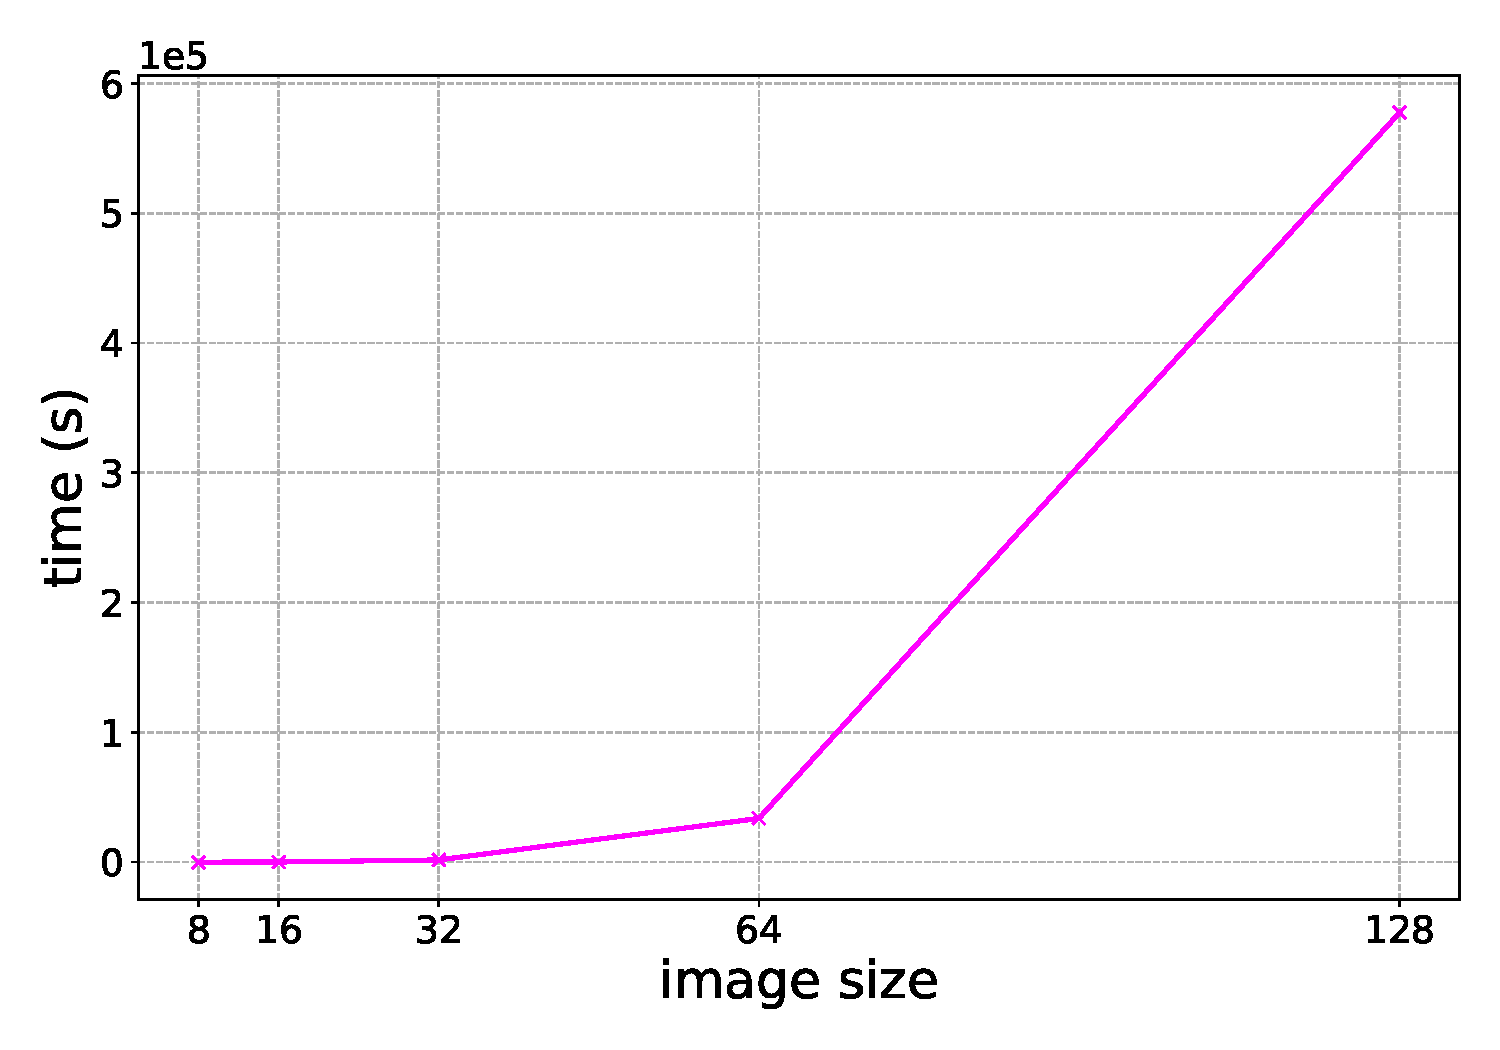
\includegraphics[width=1\columnwidth]{figures/conv_unroll}
\par\end{centering}
\caption{$3\times3$-kernel convolution (cf. Listing~\ref{lis:Single-filter-convolution-2-1})
full unrolling time vs. input (square) image size, with \texttt{store}-\texttt{load}
forwarding using MLIR's \texttt{-affine-scalrep} pass. Note that the
longest time is $577419\div3600\approx160$ hours (for a loop nest
with a trip count of $128\times128\times3\times3=147,456$). \label{fig:-kernel-convolution-full}}

\end{figure}
Translating \texttt{scf} dialect to python enables \texttt{BraggHLS}
to overcome this barrier by enabling us to use the python interpreter
as a \emph{symbolic interpreter}. Interpreting the resulting python
loop-nests (i.e., running the python program) while treating the arithmetic
and memory operations on SSA values as operations on symbols (i.e.,
python classes with overloaded methods) enables us to:
\begin{enumerate}
\item Partially evaluate functions of iteration variables, such as \mintinline{mlir}!%3 = arith.addi %i3, %i6!,
which enables concretely determining array index operands of all stores
and loads, such as \mintinline[fontsize={\small}]{mlir}!memref.load %input[%i1,%i5,%i3,%3,%4]!,
and thereupon performing memory dependence checks, thus transforming
the problem of statically verifying memory dependence into a matter
of checking assertions at runtime;
\item Unroll loops by recording each floating-point arithmetic operation
executed while enforcing SSA; e.g., for a loop whose body has repeated
assignments to the same SSA value (ostensibly violating SSA), we execute
the loop and instantiate new, uniquely identified, symbols for the
result of each operation;
\item Reconstruct all data flow through arithmetic operations and memory
operations by interpreting \texttt{memref}s as \emph{geometric symbol
tables} (i.e., symbol tables indexed by array indices rather than
identifiers/names) and \texttt{store}s and \texttt{load}s as reads
and writes on those symbol tables;
\item Easily swap evaluation rules in order to support various functional
modes, e.g., evaluating the floating-point arithmetic operations using
(python) bindings to FloPoCo's C++ functional models thereby enabling
behavioral verification of our designs.
\end{enumerate}
See Table~\ref{tab:scf-dialect-to} for the translation rules from
MLIR dialects to python.

{\scriptsize{}}
\begin{table*}[tbh]
\begin{centering}
{\scriptsize{}\caption{\texttt{scf}, \texttt{arith}, and \texttt{memref} dialect to python
translation.\label{tab:scf-dialect-to}}
}%
\begin{tabular}{ll}
\toprule
$\left\llbracket \texttt{MLIR}\right\rrbracket $ & {\small{}python}\tabularnewline
\midrule
\mintinline{mlir}!|$\llbracket$|%5|$\rrbracket$|! & \mintinline{python}!v5 = Val("%5")!\tabularnewline
\addlinespace[1mm]
\mintinline{mlir}!|$\llbracket$|memref<|$b\times c_{in}\times h\times w$|>|$\rrbracket$|! & \mintinline{python}!MemRef(|$b$|, |$c_{in}$|, |$h$|, |$w$|)!\tabularnewline
\addlinespace[1mm]
\mintinline{mlir}!|$\llbracket$||$\perc$|5 = memref.load %input[%i1, %i5, %3, %4]|$\rrbracket$|! & \mintinline{python}!|$\llbracket$|%5|$\rrbracket$| = |$\llbracket$|%input|$\rrbracket$|.__getitem__((|$\llbracket$|%i1|$\rrbracket$|, |$\llbracket$|%i5|$\rrbracket$|, |$\llbracket$|%3|$\rrbracket$|, |$\llbracket$|%4|$\rrbracket$|))!\tabularnewline
\addlinespace[1mm]
\mintinline{mlir}!|$\llbracket$| memref.store %9, %output[%i1, %i5, %3, %4]|$\rrbracket$|! & \mintinline{python}!|$\llbracket$|%output|$\rrbracket$|.__getitem__((|$\llbracket$|%i1|$\rrbracket$|, |$\llbracket$|%i5|$\rrbracket$|, |$\llbracket$|%3|$\rrbracket$|, |$\llbracket$|%4|$\rrbracket$|), |$\llbracket$|%9|$\rrbracket$|)!\tabularnewline
\addlinespace[1mm]
\mintinline{mlir}!|$\llbracket$| scf.for %i1 = %c0 to |$b$| step %c1|$\rrbracket$|! & \mintinline{python}!for |$\llbracket$|%i1|$\rrbracket$| in range(|$\llbracket$|%c0|$\rrbracket$|, |$b$|, |$\llbracket$|%c1|$\rrbracket$|)!\tabularnewline
\addlinespace[1mm]
\mintinline{mlir}!|$\llbracket$||$\perc$|3 = arith.addi %i3, %i6|$\rrbracket$|! & \mintinline{python}!|$\llbracket$|%3|$\rrbracket$| = |$\llbracket$|%i3|$\rrbracket$| + |$\llbracket$|%i6|$\rrbracket$|!\tabularnewline
\addlinespace[1mm]
\mintinline{mlir}!|$\llbracket$||$\perc$|8 = arith.mulf %5, %6|$\rrbracket$|! & \mintinline{python}!|$\llbracket$|%8|$\rrbracket$| = |$\llbracket$|%5|$\rrbracket$|.__mul__(|$\llbracket$|%6|$\rrbracket$|)!\tabularnewline
\addlinespace[1mm]
\mintinline{mlir}!|$\llbracket$||$\perc$|9 = arith.addf %7, %8|$\rrbracket$|! & \mintinline{python}!|$\llbracket$|%9|$\rrbracket$| = |$\llbracket$|%7|$\rrbracket$|.__add__(|$\llbracket$|%8|$\rrbracket$|)!\tabularnewline
\addlinespace[1mm]
\multicolumn{2}{c}{%
\begin{tabular}{ccc}
\multicolumn{1}{c}{\mintinline{mlir}!|$\llbracket$||$\perc$|63 = arith.cmpfugt |$\perc$|10, |$\perc$|c0|$\rrbracket$|!} & $\wedge$ & \multicolumn{1}{c}{\mintinline{mlir}!|$\llbracket$||$\perc$|63 = arith.cmpfugt |$\perc$|10, |$\perc$|c0|$\rrbracket$|!}\tabularnewline
\noalign{\vskip1mm}
\hline
\noalign{\vskip1mm}
\multicolumn{3}{c}{\mintinline{python}!|$\llbracket$||$\perc$|64|$\rrbracket$|.relu(|$\llbracket$||$\perc$|10|$\rrbracket$|)!}\tabularnewline
\end{tabular}}\tabularnewline
\addlinespace[1mm]
\multicolumn{2}{c}{%
\begin{tabular}{ccc}
\multicolumn{1}{c}{\mintinline{mlir}!|$\llbracket$||$\perc$|8 = arith.mulf |$\perc$|5, |$\perc$|6|$\rrbracket$|!} & $\wedge$ & \multicolumn{1}{c}{\mintinline{mlir}!|$\llbracket$||$\perc$|9 = arith.addf |$\perc$|7, |$\perc$|8|$\rrbracket$|!}\tabularnewline
\noalign{\vskip1mm}
\hline
\noalign{\vskip1mm}
\multicolumn{3}{c}{\mintinline{python}!|$\llbracket$||$\perc$|9|$\rrbracket$| = fma(|$\llbracket$||$\perc$|5|$\rrbracket$|, |$\llbracket$||$\perc$|6|$\rrbracket$|, |$\llbracket$||$\perc$|7|$\rrbracket$|)!}\tabularnewline
\end{tabular}}\tabularnewline
\bottomrule
\addlinespace[1mm]
\end{tabular}{\scriptsize\par}
\par\end{centering}
\begin{lyxcode}
\end{lyxcode}
\end{table*}
{\scriptsize\par}

\subsection{AST transformations and behavioral verification\label{subsec:AST-transformations-and-1}}

Prior to interpretation, \texttt{BraggHLS} performs some simple AST
transformations on the python generated from \texttt{scf} dialect:
\begin{enumerate}
\item \textbf{Hoist globals}: all DNN tensors which are fixed (i.e., weights)
are moved out of the body of the generated python function\footnote{\texttt{BraggHLS} translates the MLIR \texttt{module} corresponding
to the DNN into a single python function in order to simplify analysis
and interpretation.} and into the parameter list, for the purpose of ultimately exposing
them at the RTL module interface;
\item \textbf{Remove }\texttt{\textbf{if}}\textbf{ expressions}: DNN \texttt{relu}
operations are lowered to the \texttt{scf} dialect as a decomposition
into \texttt{arith.cmpfugt} and \texttt{arith.select}; this transformation
recomposes them into a \texttt{relu};
\item \textbf{Remove MACs}: sequences of \texttt{load}-\texttt{multiply}-\texttt{add}-\texttt{store}
are very common in DNN implementations, thus we schedule such sequences
jointly (this transformation coalesces such sequences into a single
\texttt{fmac} operation);
\item \textbf{Reduce }\texttt{\textbf{for}}\textbf{s}: this transformation
implements the reduction tree structure for non-parallelizable loop-nests
mentioned in Section~\ref{subsec:Scheduling}.
\end{enumerate}
These transformations on the python AST are simple (implemented with
procedural pattern matching), extensible, and efficient (marginal
runtime cost) because they are unverified: no effort is made to verify
their formal correctness. Thus, \texttt{BraggHLS} trades formal correctness
for development time performance. This tradeoff enables quick design
space iteration, which for example, enabled us to achieve very low
latency implementations for \texttt{BraggNN} (see Section~\ref{sec:BraggNN-case-study}).
As a substitute for formal verification, \texttt{BraggHLS} supports
behavioral verification. Specifically, \texttt{BraggHLS} can generate
testbenches for all synthesized RTL. The test vectors for these testbenches
are generated by evaluating the generated python representation of
the DNN on randomly generated inputs but with floating-point operations
now evaluated using functional models of the corresponding FloPoCo
operators. The testbenches can then be run using any IEEE 1364 compliant
simulator. For example, we run a battery of such testbenches (corresponding
to various DNN operation types), using \texttt{cocotb}~\cite{rosser2018cocotb}
and \texttt{iverilog}~\cite{williamsicarus}, as a part of our continuous
integration process.

\subsection{Scheduling\label{subsec:Scheduling}}

Recall that one of the critical functions which HLS fulfills is the
scheduling of operations during each clock cycle, in such a way that
they preserve the data-flow graph of a DNN; that schedule then informs
the construction of a corresponding FSM. As already mentioned, scheduling
arbitrary DNNs involves formulating and solving an ILP. In the resource-unconstrained
case, due to the precedence relations induced by data-flow, the constraint
matrix of the associated ILP is a \emph{totally unimodular matrix}
and the feasible region of the problem is an integral polyhedron.
Thus, in such cases, the scheduling problem can be solved optimally
in polynomial time with a LP solver~\cite{tuprints9272}. In the resource-constrained
case it is possible to transform resource constraints into precedence
constraints as well, by picking a particular (possibly heuristic)
linear ordering on the resource-constrained operations. This transformation
partitions resource constrained operations into distinct clock cycles,
thereby guaranteeing sufficient resources are available for all operations
scheduled within the same clock cycle~\cite{10.1145/3174243.3174268}.

\texttt{BraggHLS} uses the explicit parallelism of the \texttt{scf.parallel}
loop-nest representation to inform such a linear ordering on resource-constrained
operations. By assumption, for loop-nests which can be reprepresented
as \texttt{scf.parallel} loop-nests (see Listing~\ref{lis:Single-filter-convolution-2-2}),
each instance of a floating-point arithmetic operation in the body
corresponding to unique values of the iteration variables (e.g., \texttt{\%i1},\texttt{
\%i2},\texttt{ \%i3},\texttt{ \%i4} for Listing~\ref{lis:Single-filter-convolution-2-2})
is independent of all other such instances\footnote{Data-flow within a loop body must still be respected.}.
This exactly determines total resource usage per loop-nest; for example,
the convolution in Listing~\ref{lis:Single-filter-convolution-2-2},
would bind to $2K_{i}$ DSPs (assuming \texttt{mulf}, \texttt{addf}
bind to one DSP each), where
\begin{multline*}
K_{i}\coloneqq\left|\left\{ \texttt{\%i1}=\texttt{\%c0}+\texttt{\%c1}\times\mathbb{N}\,\wedge\,\texttt{\%i1}<b\right\} \right|\times\\
\left|\left\{ \texttt{\%i2}=\texttt{\%c0}+\texttt{\%c1}\times\mathbb{N}\,\wedge\,\texttt{\%i2}<c_{out}\right\} \right|\times\\
\left|\left\{ \texttt{\%i3}=\texttt{\%c0}+\texttt{\%c1}\times\mathbb{N}\,\wedge\,\texttt{\%i3}<h\right\} \right|\times\\
\left|\left\{ \texttt{\%i4}=\texttt{\%c0}+\texttt{\%c1}\times\mathbb{N}\,\wedge\,\texttt{\%i4}<w\right\} \right|
\end{multline*}
where $\texttt{\%c1}\times\mathbb{N}$ represents all multiples of
$\texttt{\%c1}$. That is to say, $K_{i}$ is the cardinality of the
cartesian product of the iteration spaces of the parallel iteration
variables.
\begin{listing}
\begin{minted}[fontsize={\scriptsize},escapeinside={||},mathescape=true]{mlir}
@conv2d(
    %input: memref<|$b \times c_{in} \times h \times w$|>,
    %weight: memref<|$b \times c_{out} \times h \times w$|>,
    %output: memref<|$c_{out} \times c_{in} \times k \times k$|>
) {
  scf.parallel (%i1, %i2, %i3, %i4) =
               (%c0, %c0, %c0, %c0) to
               (|$b$|, |$c_{out}$|, |$h$|, |$w$|) step
               (%c1, %c1, %c1, %c1) {
    scf.for %i5 = %c0 to |$c_{in}$| step %c1 {
      scf.for %i6 = %c0 to |$k$| step %c1 {
        scf.for %i7 = %c0 to |$k$| step %c1 {
          %3 = arith.addi %i3, %i6
          %4 = arith.addi %i4, %i7
          %5 = memref.load %input[%i1, %i5, %i3, %3, %4]
          %6 = memref.load %weight[%i2, %i5, %i6, %i7]
          %7 = memref.load %output[%i1, %i2, %i3, %i4]
          %8 = arith.mulf %5, %6
          %9 = arith.addf %7, %8
          memref.store %9, %output[%i1, %i2, %i3, %i4]
        }
      }
    }
  }
  return %2
}
\end{minted}
\caption{Parallel loop representation of the convolution in Listing~\ref{lis:Single-filter-convolution}.\label{lis:Single-filter-convolution-2-2}}
\end{listing}
. Taking the maximum over such $K\coloneqq\max_{i}K_{i}$ across all \texttt{scf.parallel}
loop-nests, we can infer peak usage of any resource. Then, after indexing
available hardware resources $j=1,\dots,K$, we can bind the operations
of any particular loop-nest. This leads to a linear ordering on resource-constrained
operations such that operations bound to the same hardware resource
index $j$ must be ordered according to their execution order during
symbolic interpretation\footnote{\texttt{BraggHLS} only needs to construct a partial precedence ordering
$\texttt{op}_{a}<\texttt{op}_{b}$ for operations $\texttt{op}_{a},\texttt{op}_{b}$
which CIRCT then combines with the delays of the operations to construct
constraints such as $\texttt{start\_op}_{a}+\texttt{delay}_{a}\leq\texttt{start\_op}_{b}$.}. Note, this ordering coincides with the higher-level structure of
the DNN, since ordering of\texttt{ scf.parallel} loop nests (and thus
interpretation order during execution of the python program) is determined
by the higher-level structure of the DNN.

For DNN operations that do not lower to \texttt{scf.parallel} loop-nests
but do lower to sequential loop nests (e.g., \texttt{sum}, \texttt{max},
or \texttt{prod}), we fully unroll the loops and transform the resulting,
sequential, operations into a reduction tree; we use As-Late-As-Possible
scheduling~\cite{baruch1996scheduling} amongst the subtrees of such
reduction trees.

\section{Evaluation\label{sec:Evaluation}}

We evaluate \texttt{BraggHLS} both on individual DNN layers, and end-to-end,
on our use-case \texttt{BraggNN}. We compare \texttt{BraggHLS} to
Xilinx's Vitis HLS by comparing the latencies and resource usages
of the final designs generated by each. We also compare the runtimes
of the tools themselves. Both \texttt{BraggHLS} and Vitis HLS produce
Verilog RTL, on which we run a synthesis pass using Xilinx's Vivado.
The particular FPGA target is Xilinx Alveo U280. We measure LUT, DSP,
BRAM, and FF usage. For the DNN layer evaluations, we use FloPoCo
$\left(5,11\right)$-floating point representations (5 bits for the
exponent and 11 bits for the mantissa) corresponding to Vitis HLS's
IEEE half precision IPs. We synthesize all designs for a 10 ns target
clock period and report end-to-end latency as a product of the total
schedule interval count of the design and achieved clock period ($10-WNS$,
where $WNS$ is the worst negative slack reported). Note, in the case
of Vitis HLS, which potentially explicitly pipelines the design and
therefore implements with an initiation interval strictly less than
the total schedule interval count, we report in terms of the best
possible interval count (\texttt{LatencyBest} from the Vitis HLS reports).
All other measurements are collected from Vivado synthesis reports.
Note, since Vitis HLS operates on C++ representations, we generate
such a representation for our test cases by first lowering each DNN
layer to the \texttt{affine} dialect and then using the \texttt{scalehls-translate}
tool of the ScaleHLS project~\cite{yehpca2022scalehls} to emit C++.
Importantly, we do not make any use of \texttt{scalehls-opt} optimization
tool (of the same project).

Since our ultimate goal is low latency inference, and since the strategy
that \texttt{BraggHLS} employs in the pursuit of this goal is loop
unrolling, in order to produce a like for like comparison, we similarly
unroll the representation that is passed to Vitis HLS. Thus, all Vitis
HLS measurements are reported in terms of \emph{unroll factor}: an
unroll factor of $k$ corresponds to a $k$-fold increase in the number
of statements in the body of a loop and commensurate $k$-fold decrease
in the trip count of the loop. For loop nests we unroll inside out:
if $k$ is greater than the trip count $t$ of the innermost loop,
we unroll the innermost loop completely and then unroll the enclosing
loop by a factor of $k-t$. We do not perform any store-load forwarding
during this preprocessing but we annotate all arrays with the directive
\mintinline{tex}!array_partition complete dim=1! in order that Vitis
HLS can effectively pipeline. All representations generated by \texttt{BraggHLS}
correspond to full unrolling of the loop nests.

\subsection{DNN layers}

See Figure~\ref{fig:Resource-usage-and}; we evaluate \texttt{BraggHLS}
against Xilinx's Vitis HLS by comparing the latency of the final design
on the following, individual, DNN layer types:
\begin{itemize}
\item \mintinline{python}!addmm(a, b, c)!: Matrix multiplication of the
matrices \texttt{a} and \texttt{b}. The matrix \texttt{c} is added
to the final result;
\item \mintinline{python}!batch_norm_2d(num_features)!: Batch Normalization
over a 4D input as described in~\cite{https://doi.org/10.48550/arxiv.1502.03167};
\item \mintinline{python}!conv_2d(|$c_{in}$|, |$c_{out}$|, |$k$|)!: 2D
convolution with bias, with $k\times k$ kernel, over a $b\times c_{in}\times h\times w$
input, producing $b\times c_{out}\times h'\times w'$ output;
\item \mintinline{python}!max_pool_2d(|$k$|, stride)!: 2D max pooling,
with $k\times k$ kernel, and striding;
\item \mintinline{python}!soft_max!: The softmax function
\[
\text{softmax}\left(\boldsymbol{x}\right)\coloneqq\left[\frac{\exp\left(x_{i}\right)}{\sum_{j}\exp\left(x_{j}\right)}\right]
\]
\end{itemize}
The layers were chosen to cover a range of arithmetic operations (\texttt{mulf},
\texttt{divf}, \texttt{addf}, \texttt{subf}, \texttt{sqrtf}) and data
access patterns (iteration, accumulation, and reduction). The concrete
parameter values and dimensions of inputs used during evaluation are
summarized in Table~\ref{tab:Resource-usage-for-2}.
\begin{table*}[tbh]
\caption{DNN layers used for evaluation of \texttt{BraggHLS.} \label{tab:Resource-usage-for-2}}

\centering{}%
\begin{tabular}{lll}
\toprule
Layer & Parameter values & Input dimensions\tabularnewline
\midrule
\mintinline{python}!addmm! & N/A & $\dim\left(\texttt{a}\right)=\dim\left(\texttt{b}\right)=\dim\left(\texttt{c}\right)=\left(16,16\right)$\tabularnewline
\midrule
\mintinline{python}!batch_norm_2d! & $\texttt{num\_features}=2$ & $\dim\left(\texttt{input}\right)=\left(10,2,3,3\right)$\tabularnewline
\midrule
\mintinline{python}!conv_2d! & $c_{in}=1,c_{out}=3,k=3$ & $\dim\left(\texttt{input}\right)=\left(1,1,16,16\right)$\tabularnewline
\midrule
\mintinline{python}!max_pool_2d! & $k=3,\texttt{stride}=2$ & $\dim\left(\texttt{input}\right)=\left(1,3,16,16\right)$\tabularnewline
\midrule
\mintinline{python}!soft_max! & N/A & $\dim\left(\texttt{input}\right)=\left(1,3,16,16\right)$\tabularnewline
\bottomrule
\end{tabular}
\end{table*}
\begin{figure*}[!t]
\begin{centering}
\subfloat[\texttt{addmm}]{\centering{}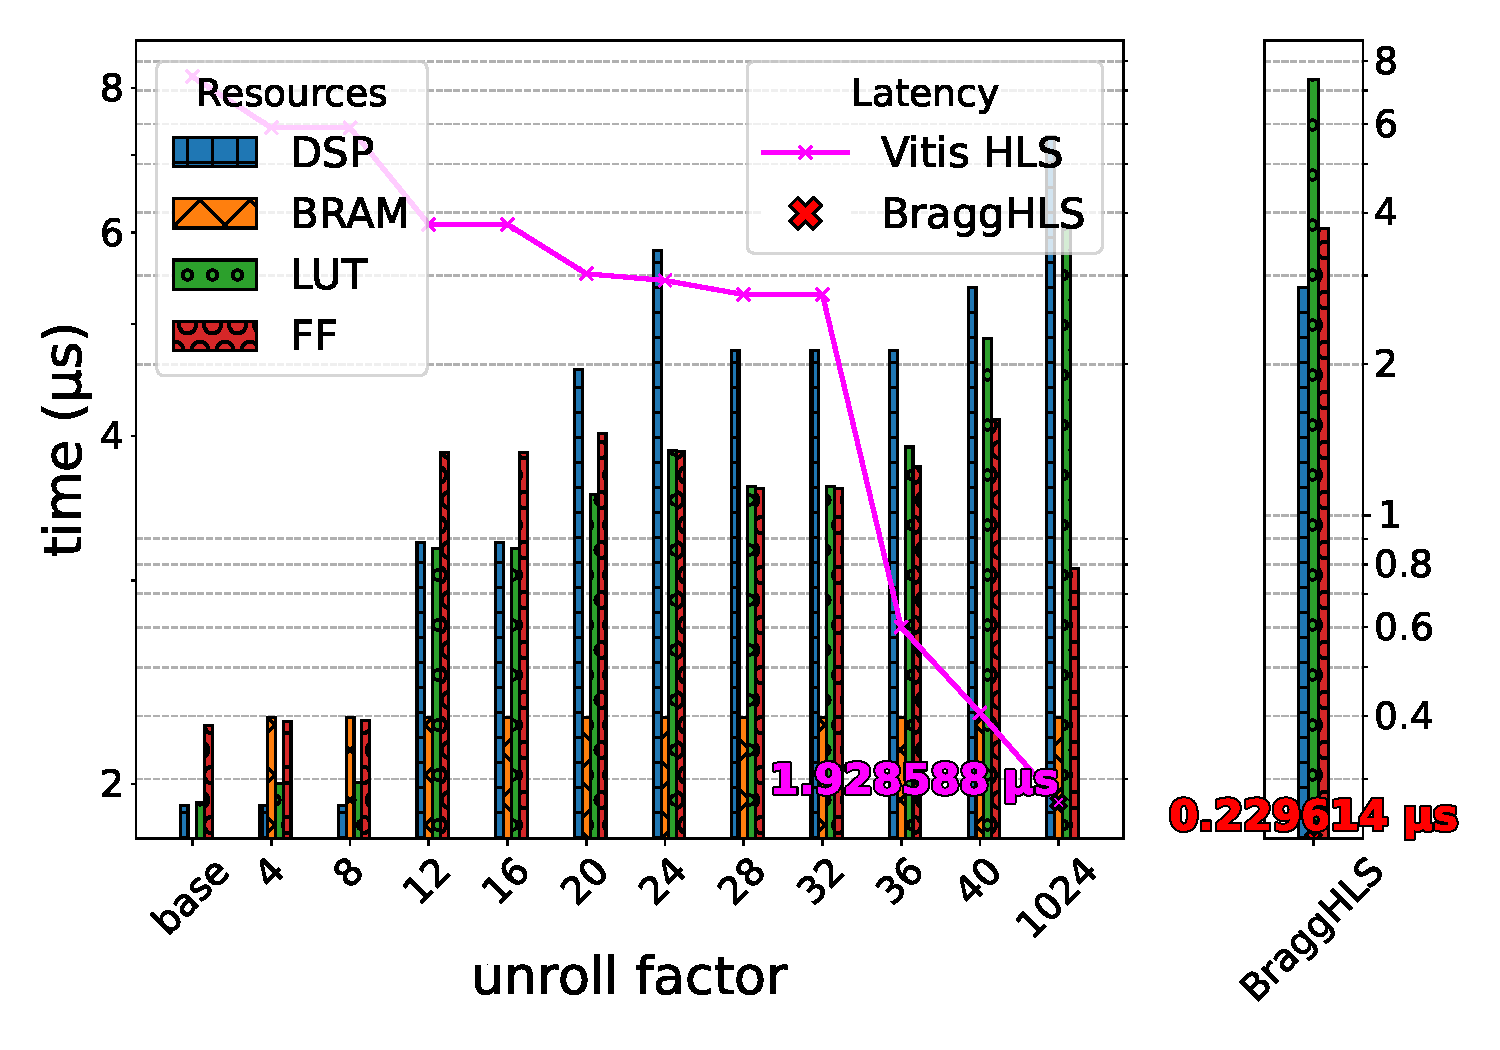
\includegraphics[width=1\columnwidth]{figures/addmm}\label{2dlattice-1-1-2}}\subfloat[\texttt{batch\_norm\_2d}]{\centering{}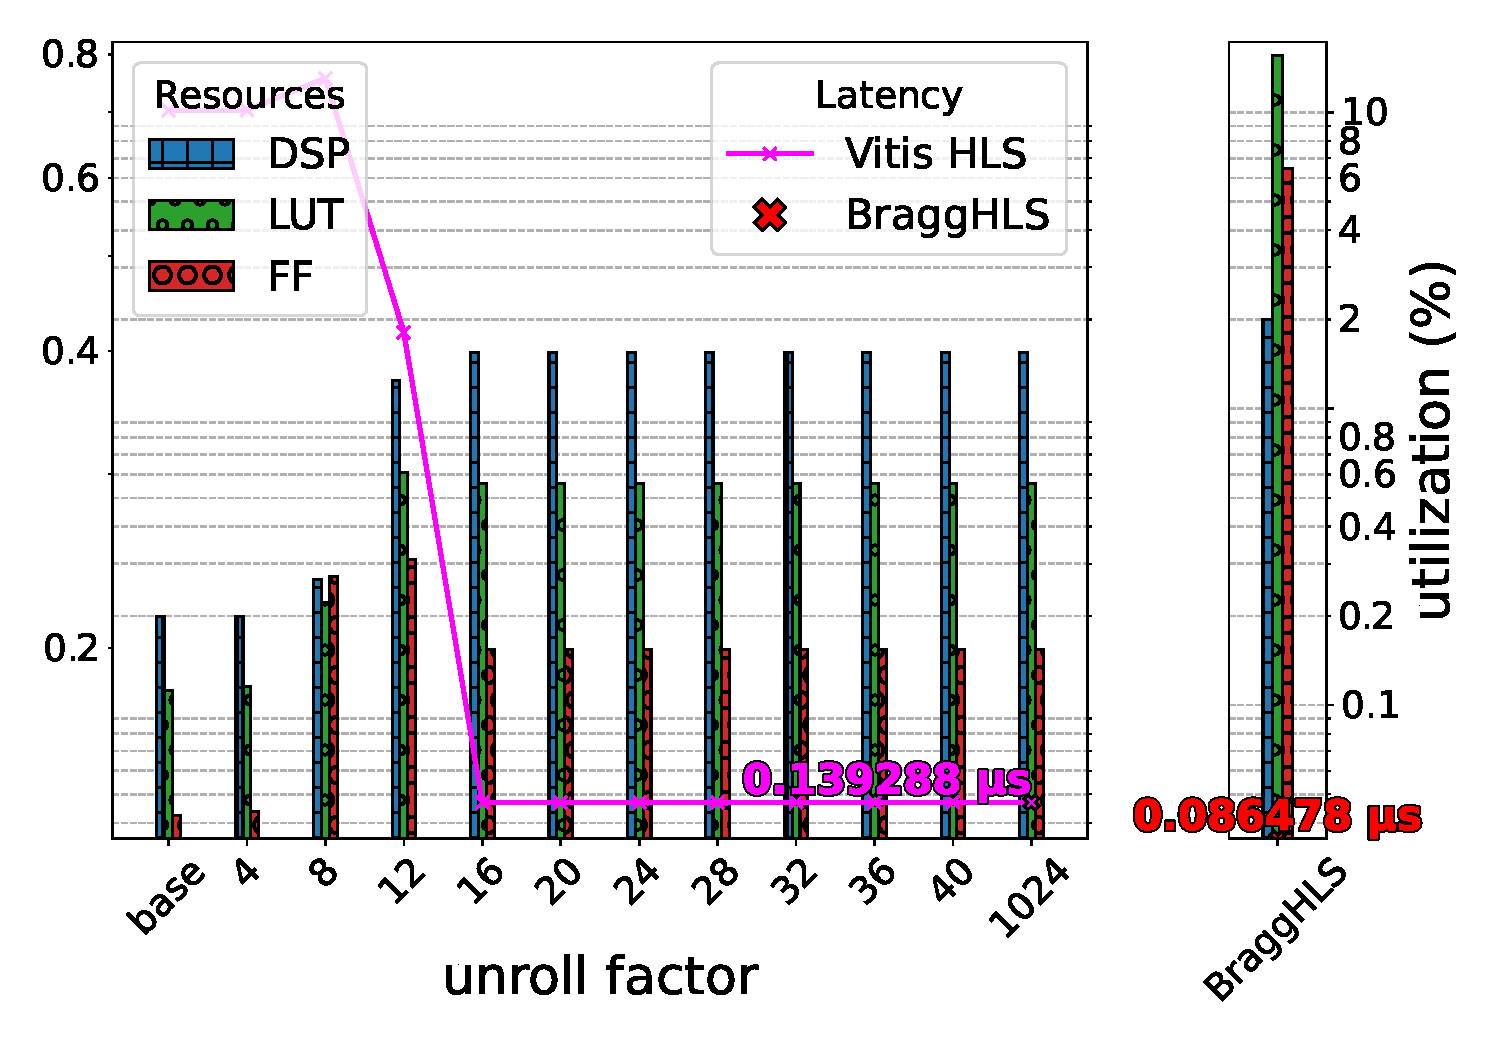
\includegraphics[width=1\columnwidth]{figures/batch_norm}\label{2dlattice-1-2-2}}
\par\end{centering}
\medskip{}

\centering{}\label{2dlattice-1-3}\subfloat[\texttt{conv\_2d}]{\centering{}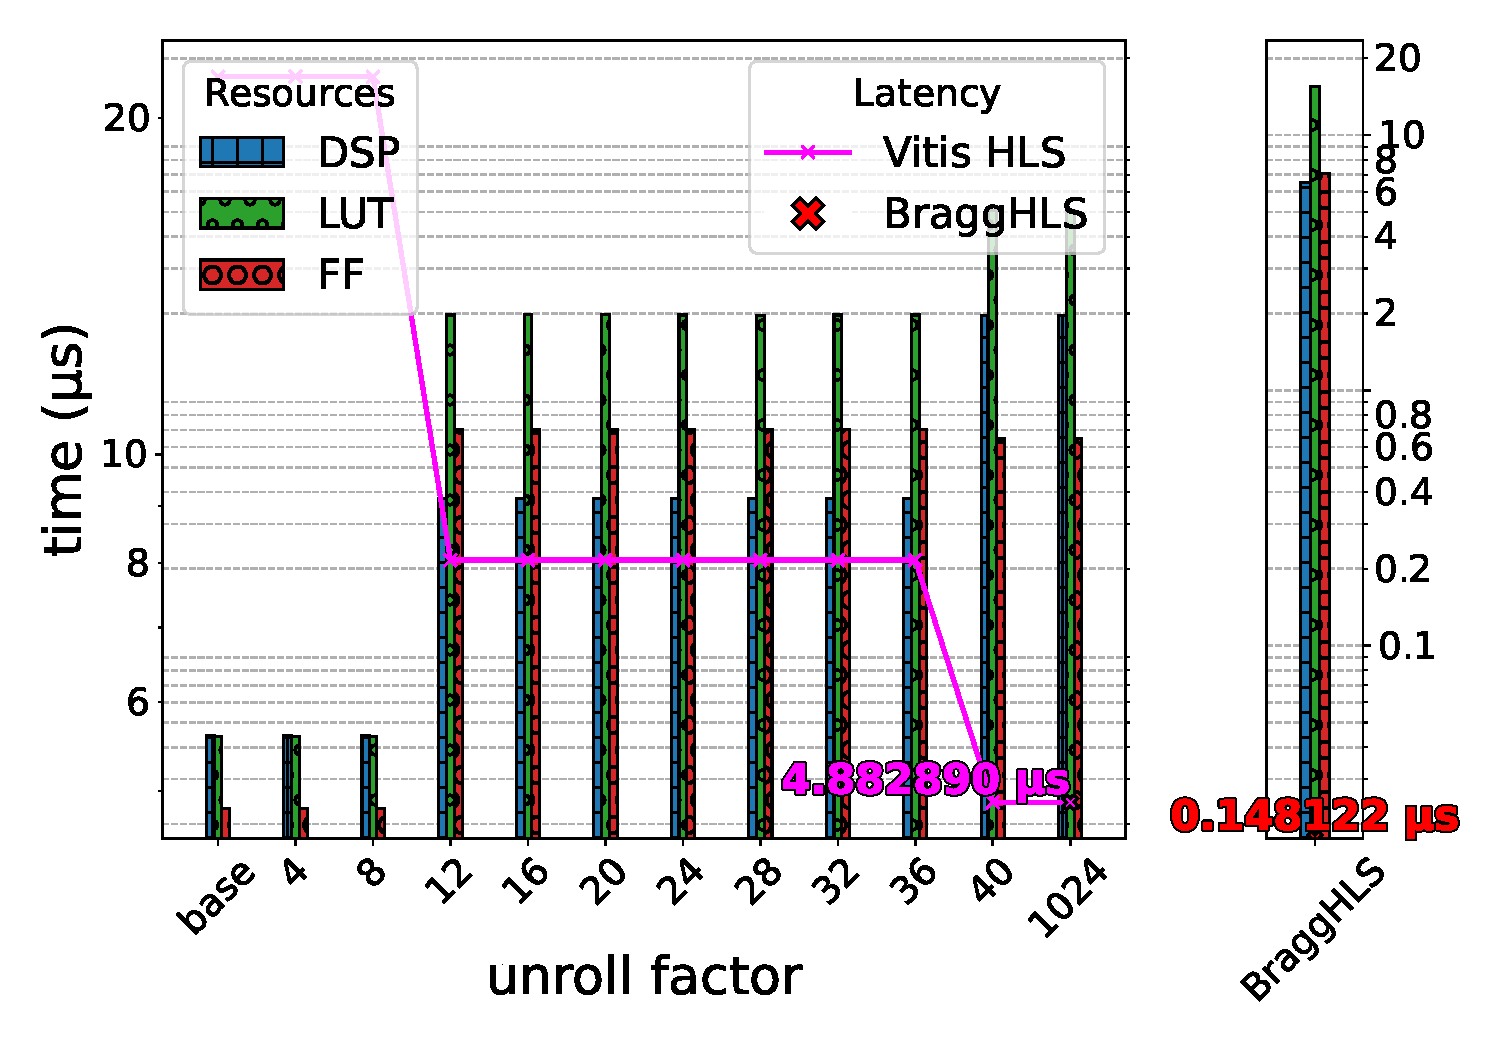
\includegraphics[width=1\columnwidth]{figures/conv}\label{2dlattice-1-1-1-1}}\subfloat[\texttt{max\_pool\_2d}]{\centering{}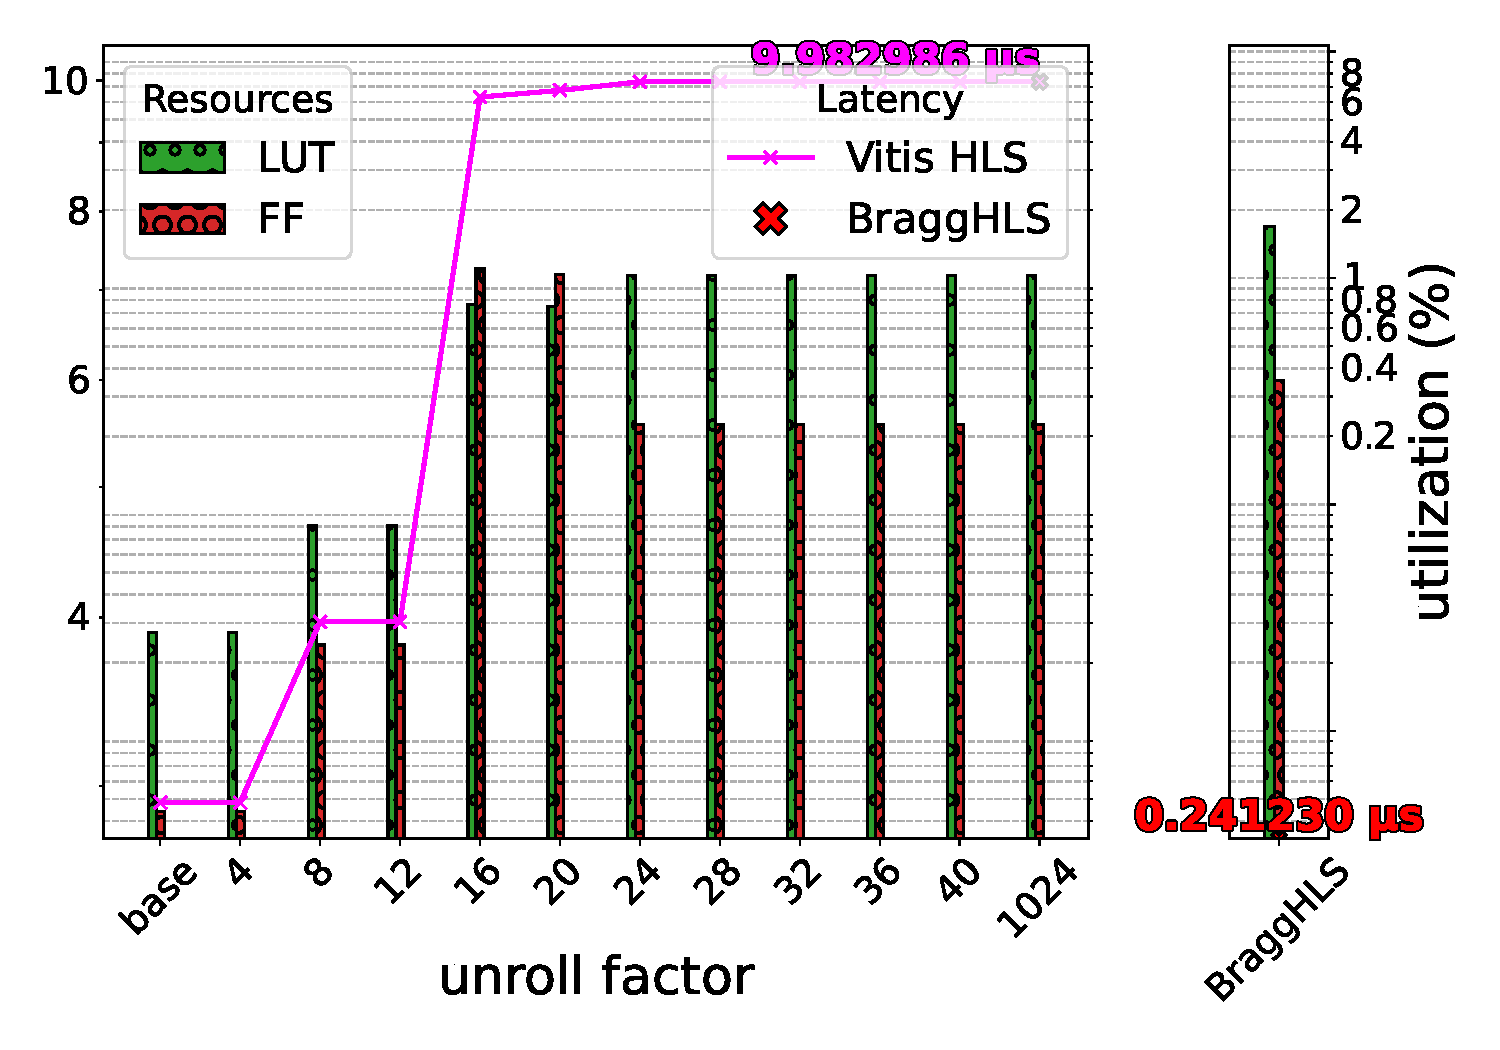
\includegraphics[width=1\columnwidth]{figures/max_pool_2d}\label{2dlattice-1-2-1-1}}\medskip{}
\subfloat[\texttt{soft\_max}]{\centering{}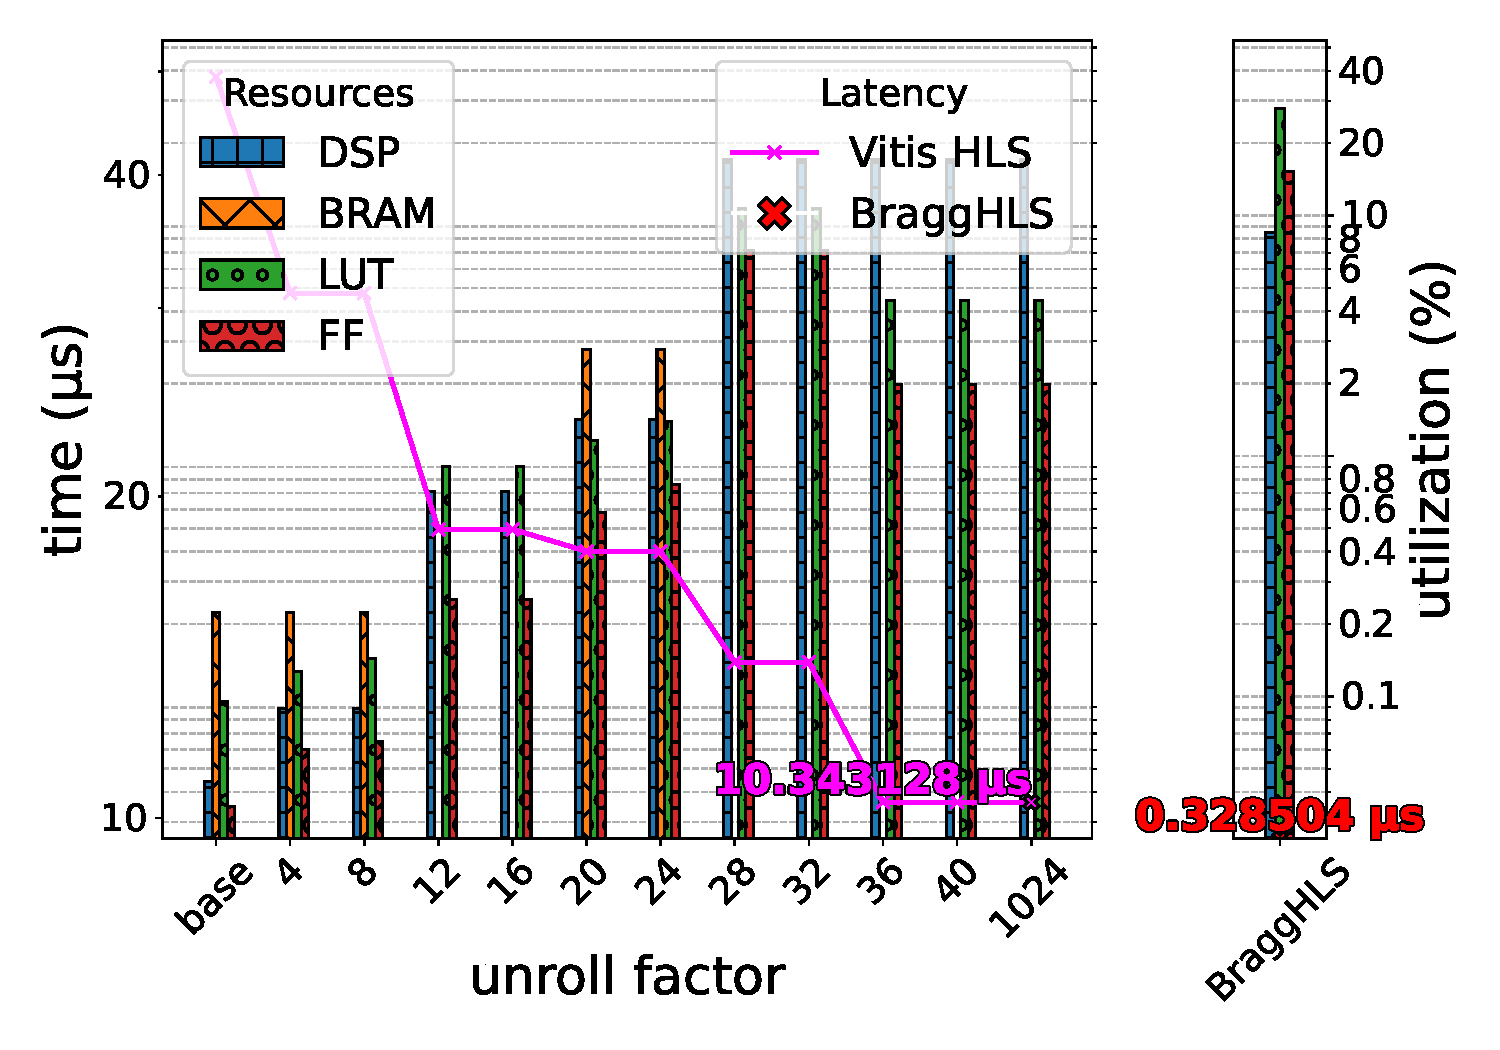
\includegraphics[width=1\columnwidth]{figures/soft_max}\label{2dlattice-1-2-1-1-1}}\caption{Vitis HLS vs. \texttt{BraggHLS} resource usage and latency vs. unroll
factor of various DNN modules. All $y$-scales are log.\label{fig:Resource-usage-and}}
\end{figure*}
\begin{figure*}[tbh]
\centering{}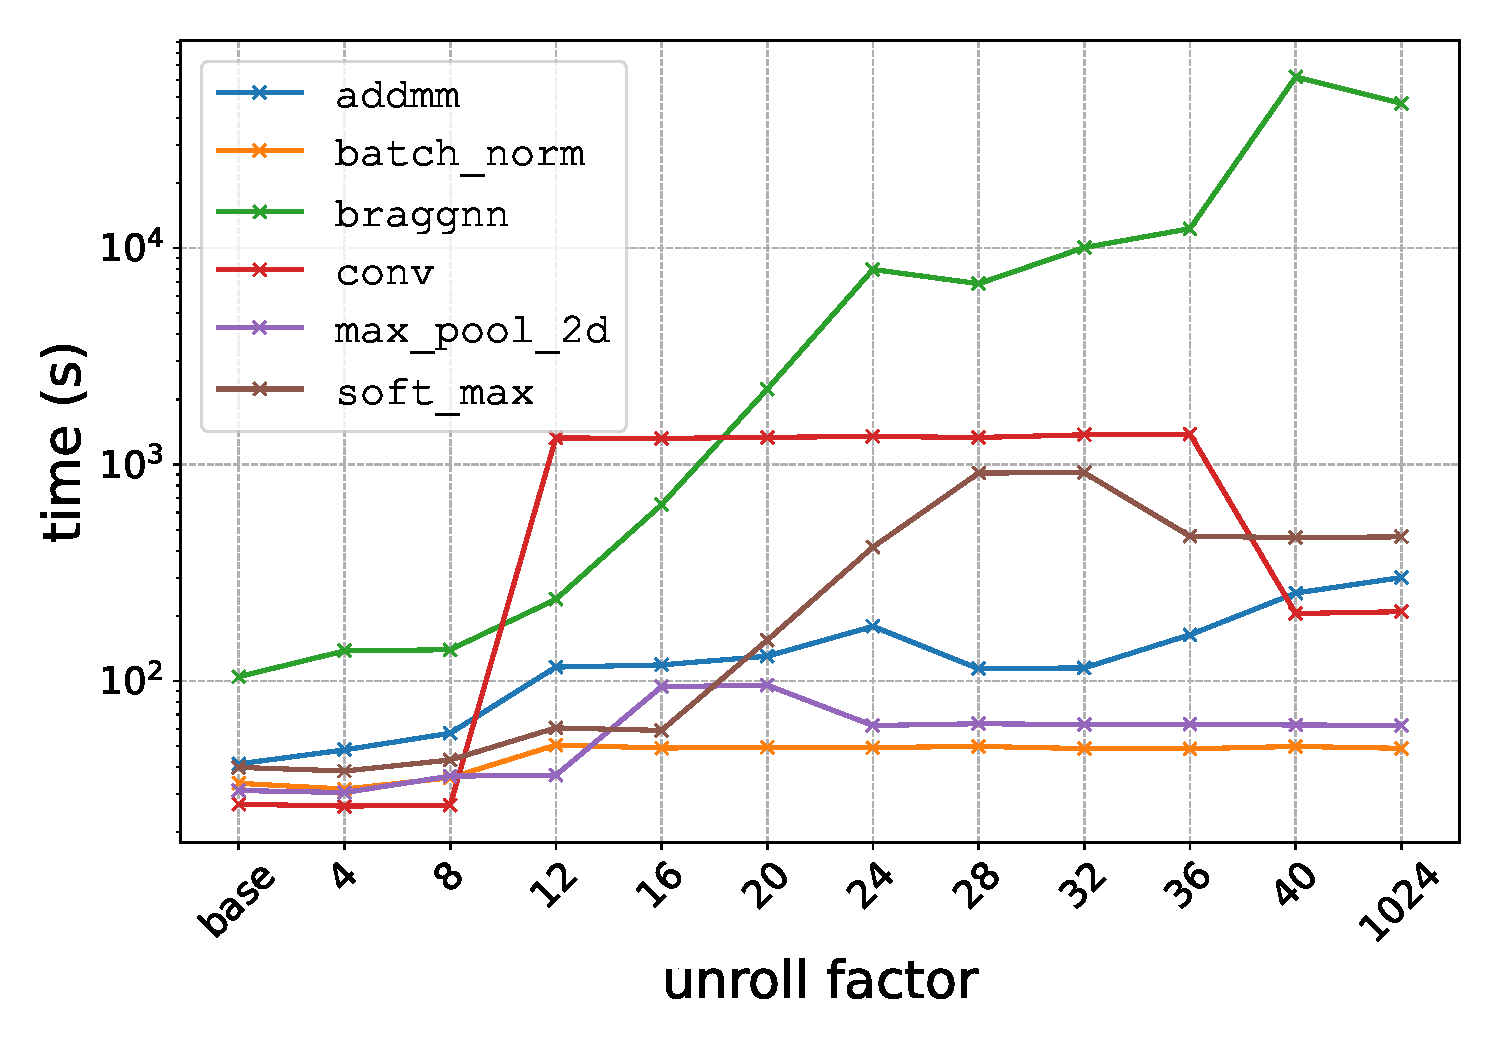
\includegraphics[width=1\columnwidth]{figures/elapsed_time}\caption{Runtime of Vitis HLS vs. unroll factor.\label{fig:Runtime-of-Vitisa}}
\end{figure*}

See Figure~\ref{fig:Resource-usage-and} for Vitis HLS vs. \texttt{BraggHLS}
resource usage and latency vs. unroll factor and Figure~\ref{fig:Runtime-of-Vitisa}
for the runtimes of Vitis HLS as function of increasing unroll factor.
We observe that Vitis HLS indeed approaches lower and lower end-to-end
latencies as a function of unroll factor but that for none of the
unroll factors is it able to match the end-to-end latency achieved
by \texttt{BraggHLS}. Even at unroll factor equal to 1024 (which corresponds
to fully unrolled for all of the loop nests comprising these layer
types), Vitis HLS is only within 10$\times$ of \texttt{BraggHLS}.
We hypothesize that in general this is due to Vitis HLS's inability
to effectively pipeline due to inability to eliminate memory dependencies,
either through \texttt{store}-\texttt{load} forwarding or further
array partitioning\footnote{Indeed Vitis HLS can be seen to produce warnings such as \colorbox{bg}{\parbox{\columnwidth}{\texttt{WARNING: [HLS 200-885] Unable to schedule 'load' operation ...
due to limited memory ports (II = 1). Please consider using a memory core with more ports or partitioning the array ...}}}}. Conversely, \texttt{BraggHLS}'s ability to effectively perform \texttt{store}-\texttt{load}
forwarding is evident in the complete lack of BRAM usage: all weights
are kept on FFs or LUTs. While this is infeasible for larger designs
(which would be constrained by the number of available FFs), for our
particular use case, this unconstrained usage of FFs is acceptable.
Note, the increasing latency (as a function of unroll factor) in the
case of \texttt{max\_pool\_2d} is due to Vitis HLS's failure to meet
timing, i.e., while the interval count decreases as a function of
unroll factor, the clock period increases (see Appendix Table~\ref{tab:all_unrolls}
for exact values).


\subsection{\texttt{BraggNN} case study\label{sec:BraggNN-case-study}}

\begin{figure}[tbh]
\centering{}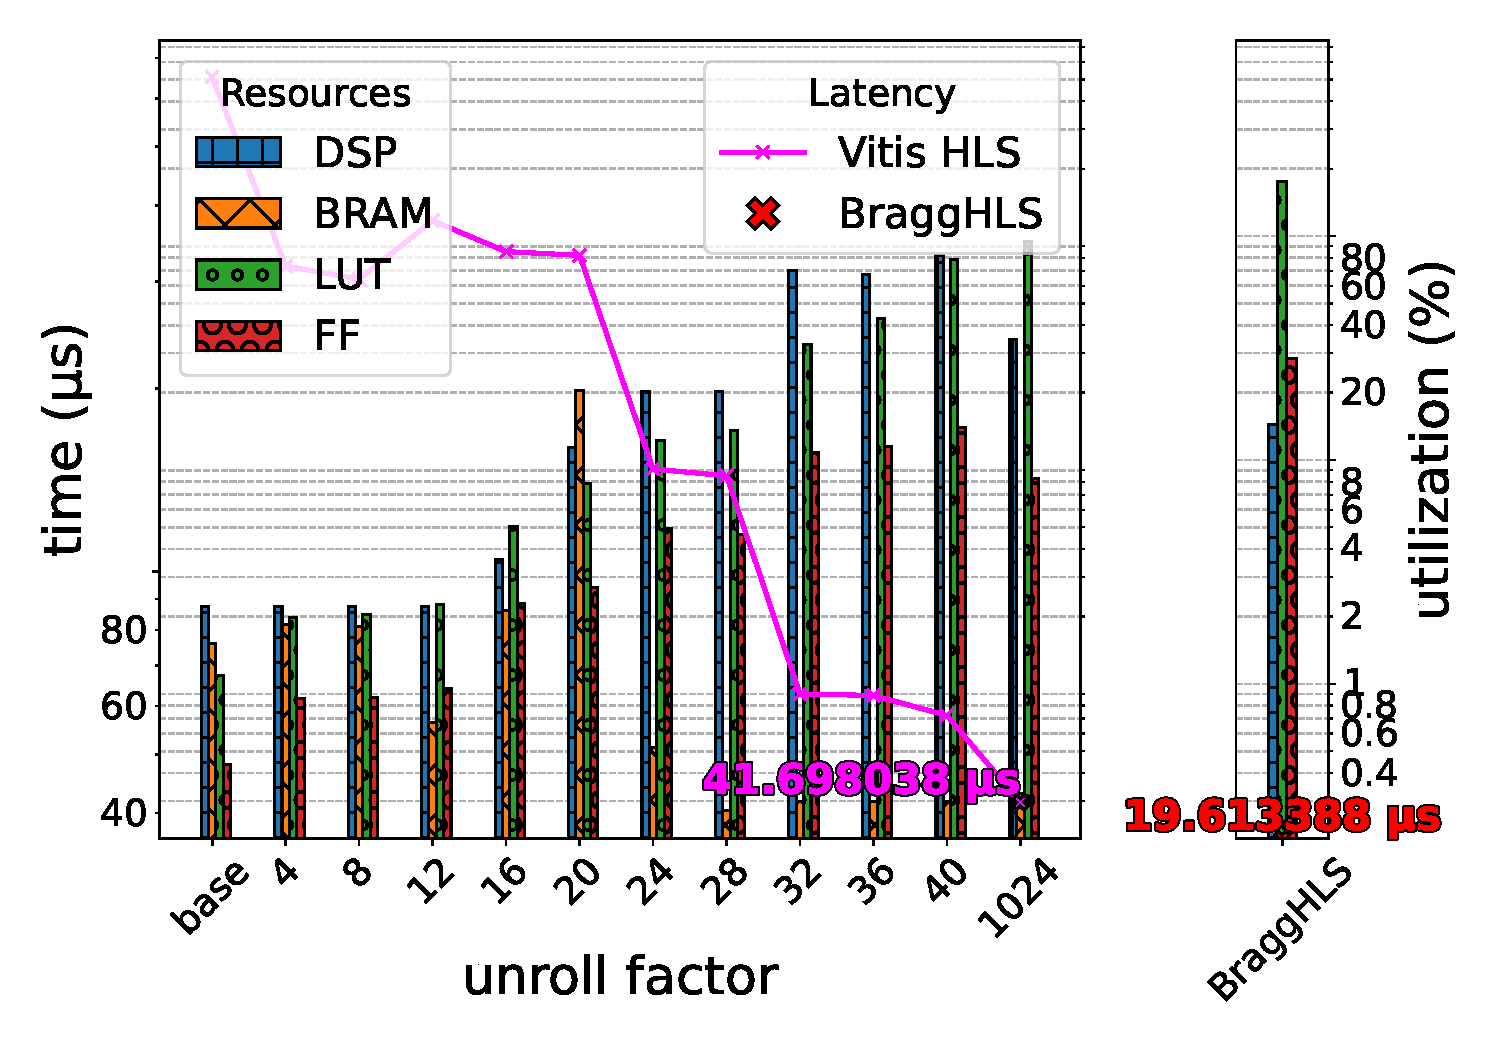
\includegraphics[width=1\columnwidth]{figures/braggnn}\caption{\texttt{BraggNN} Vitis HLS vs. \texttt{BraggHLS} resource usage and
latency vs. unroll factor.\texttt{\label{fig:braggnn}}}
\end{figure}

High-energy diffraction microscopy techniques can provide non-destructive
characterization for a broad class of single-crystal and polycrystalline
materials. The critical steps in a typical HEDM experiment involve
an analysis to determine precise Bragg diffraction peak characteristics
(followed by reconstruction of material grain information from the
peak characteristics). Peak characteristics are typically computed
by fitting the peaks to a probability distribution, e.g., Gaussian,
Lorentzian, Voigt, or Pseudo-Voigt. As already mentioned (in Section
\ref{sec:Introduction}) these experiments can have collection rates
in excess of 80 GB/s. These data rates, though more modest than those
observed at the LHC, combined with the runtime of the fitting procedure,
merit exploring the same low latency approach (as explored employed
by LHC experiments) in order to enable experiment modalities that
depend on measurement-based feedback (i.e., experiment steering).
\begin{listing}
\begin{minted}[fontsize={\scriptsize},escapeinside={||},mathescape=true]{python}
BraggNN(|$s$|)(
  (cnn_layers_1): Conv2d(|$s \times 16 $|, kernel=3, stride=1)
  (nlb): NLB(
    (theta_layer): Conv2d(|$s \times 16 $|, |$s \times 8 $|, kernel=1, stride=1)
    (phi_layer): Conv2d(|$s \times 16 $|, |$s \times 8 $|, kernel=1, stride=1)
    (g_layer): Conv2d(|$s \times 16 $|, |$s \times 8 $|, kernel=1, stride=1)
    (out_cnn): Conv2d(|$s \times 8 $|, |$s \times 16 $|, kernel=1, stride=1)
    (soft): Softmax()
  )
  (cnn_layers_2): Sequential(
    (0): ReLU()
    (1): Conv2d(|$s \times 16 $|, |$s \times 8 $|, kernel=3, stride=1)
    (2): ReLU()
    (3): Conv2d(|$s \times 8 $|, |$s \times 2 $|, kernel=3, stride=1)
    (4): ReLU()
  )
  (dense_layers): Sequential(
    (0): Linear(in_features=|$s \times 50$|, out_features=|$s \times 16 $|)
    (1): ReLU()
    (2): Linear(in_features=|$s \times 16 $|, out_features=|$s \times 8 $|)
    (3): ReLU()
    (4): Linear(in_features=|$s \times 8 $|, out_features=|$s \times 4 $|)
    (5): ReLU()
    (6): Linear(in_features=|$s \times 4 $|, out_features=2)
    (7): ReLU()
  )
)
\end{minted}
\caption{\texttt{BraggNN} for scale $s=1,2$.\label{lis:braggnn}}
\end{listing}

\texttt{BraggNN}~\cite{Liu:fs5198}, a DNN aimed at efficiently characterizing
Bragg diffraction peaks, achieves a throughput of approximately 22
\textmu s/sample (via batch inference). This is a large speedup over
the classical pseudo-Voigt peak fitting methods, but still falls far
short of the 1 \textmu s/sample target for handling the 1 MHz sampling
rates. In addition, the current implementation of \texttt{BraggNN},
deployed to either a data-center class GPU such as a NVIDIA V100,
or even a workstation class GPU such as a NVIDIA RTX 2080Ti, has no
practicable means to being deployed at the edge, i.e., adjacent or
proximal to the high energy microscopy equipment. Towards this end,
we applied \texttt{BraggHLS} to the PyTorch representation of \texttt{BraggNN($s=1$)}\emph{
}(see Listing~\ref{lis:braggnn}) and achieved a RTL implementation
which synthesizes to a 1,238 interval count design that places, routes,
and meets timing closure for a clock period of 10 ns (for a Xilinx
Alveo U280). The design consists of a three stage pipeline with the
longest stage measuring 480 intervals. Thus, the throughput of the
implementation is 4.8 \textmu s/sample. See Table~\ref{tab:Resource-usage-for}
for a summary of the resource usage of the implementation and Figure
\ref{fig:braggnn} for a comparison with designs generated by Vitis
HLS.

The most challenging aspect of implementing \texttt{BraggNN} was minimizing
latency while satisfying compute resource constraints (LUTs, DSPs,
BRAMs) and meeting routing ``closure'', i.e., not exceeding available
routing resources and avoiding congestion. Two design choices were
made for the purposes of reducing resource consumption. The first
was reducing the precision used for the floating-point operations.
We reduced the precision from half precision to FloPoCo $\left(5,4\right)$-precision
(5 bits for the exponent and 4 bits for the mantissa). This was justified
by an examination of the distribution of the weights of the fully
trained \texttt{BraggNN} (see figure~\ref{fig:BraggHLS-framework-overview.-1}).
\begin{figure}[tbh]
\centering{}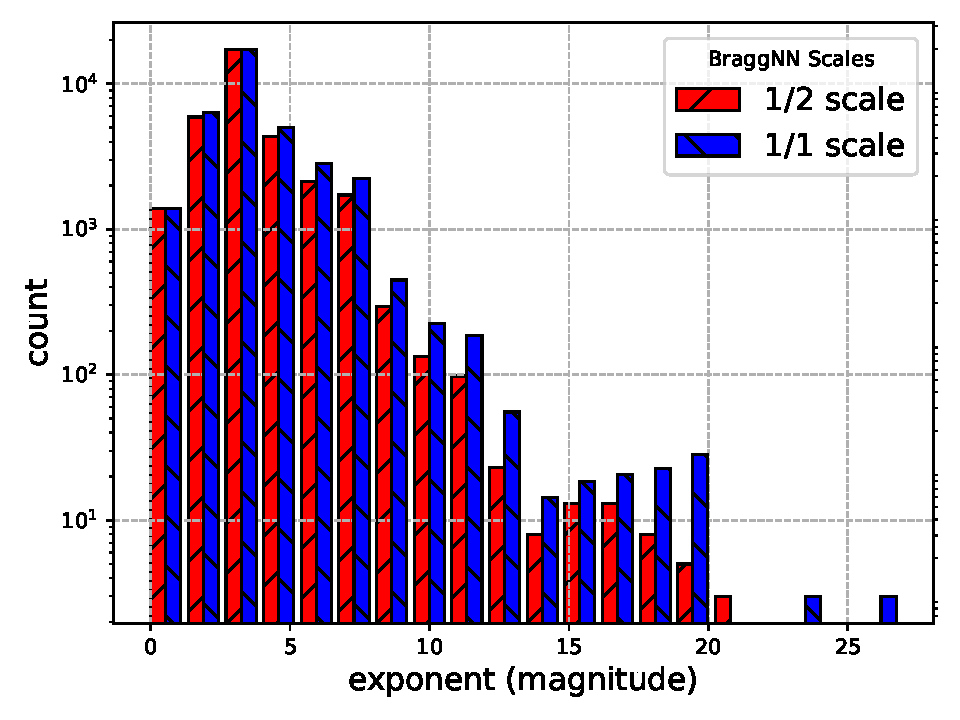
\includegraphics[width=1\columnwidth]{figures/exp_hist}\caption{\texttt{BraggHLS} weights exponent distribution.\label{fig:BraggHLS-framework-overview.-1}}
\end{figure}
 Reducing the precision enabled the second design choice: we eliminate
BRAMs from the design, since, at the lower precision, all weights
can be represented as registered constants. The reduced precision
also drives the Vivado synthesizer to infer implementations of the
floating-point operations that make no use of DSPs; this was not intentional
but seemingly cannot be altered. Most likely this is due to the fact
that the DSP48 hardware block includes a 18-bit by 25-bit signed multiplier
and a 48-bit adder~\cite{guideultrascale}, neither of which neatly
divide the bit width of FloPoCo $\left(5,4\right)$-precision cores\footnote{The actual bit width for FloPoCo $\left(5,4\right)$-precision is
12 bits: 1 extra bit is needed for the sign and 2 bits are needed
for FloPoCo's handling of exceptional conditions.}.

Achieving routing closure was very difficult due to the nature of
the Xilinx's UltraScale architecture, of which the Alveo U280 is an
instance. The UltraScale architecture achieves its scale through ``Stacked
Silicon Interconnect'' (SSI) technology~\cite{leibson2013xilinx},
which implies multiple distinct FPGA dies, called Super Logic Regions
(SLRs), on the same chip, connected by interposers. Adjacent SLRs
communicate with each other using a limited set of Super Long Lines
(SLLs). These SLLs determine the maximum bus width that spans two
SLRs. On the Alveo U280 there are exactly 23,040 SLLs available between
adjacent SLRs and at $\left(5,4\right)$-precision \texttt{BraggNN($s=1$)}
needs 23,328 SLLs between SLR2 and SLR1\footnote{We route the output of \texttt{cnn\_layers\_1} ($1\times16\times9\times9\times12$
wires) as well as the output of $\texttt{soft(theta\_layer}\times\texttt{phi\_layer)}\times\texttt{g\_layer}$
($1\times8\times9\times9\times12$ wires) from SLR2 to SLR1.}. Thus, we further reduced the precision to $\left(5,3\right)$. Finally,
since multiple dies constitute independent clock domains, the SLLs
that cross SLRS are sensitive to hold time violations due to the higher
multi-die variability~\cite{rapidwright}. This multi-die variability
leads to high congestion if not addressed. Thus, routing across SLRs
needs to be handled manually, using placement and routing constraints
for logic in each SLR and the addition of so-called ``launch'' and
``latch'' registers in each SLR. See figure~\ref{fig:BraggHLS-framework-overview.-2}
for an illustration on the effect of using launch and latch registers
as well as placement and routing constraints.
\begin{figure*}[tbh]
\centering{}\subfloat[\texttt{BraggNN} fails to achieve routing closure without placement
and routing constraints and launch and latch registers.\label{fig:BraggHLS-framework-overview.-2-1}]{\centering{}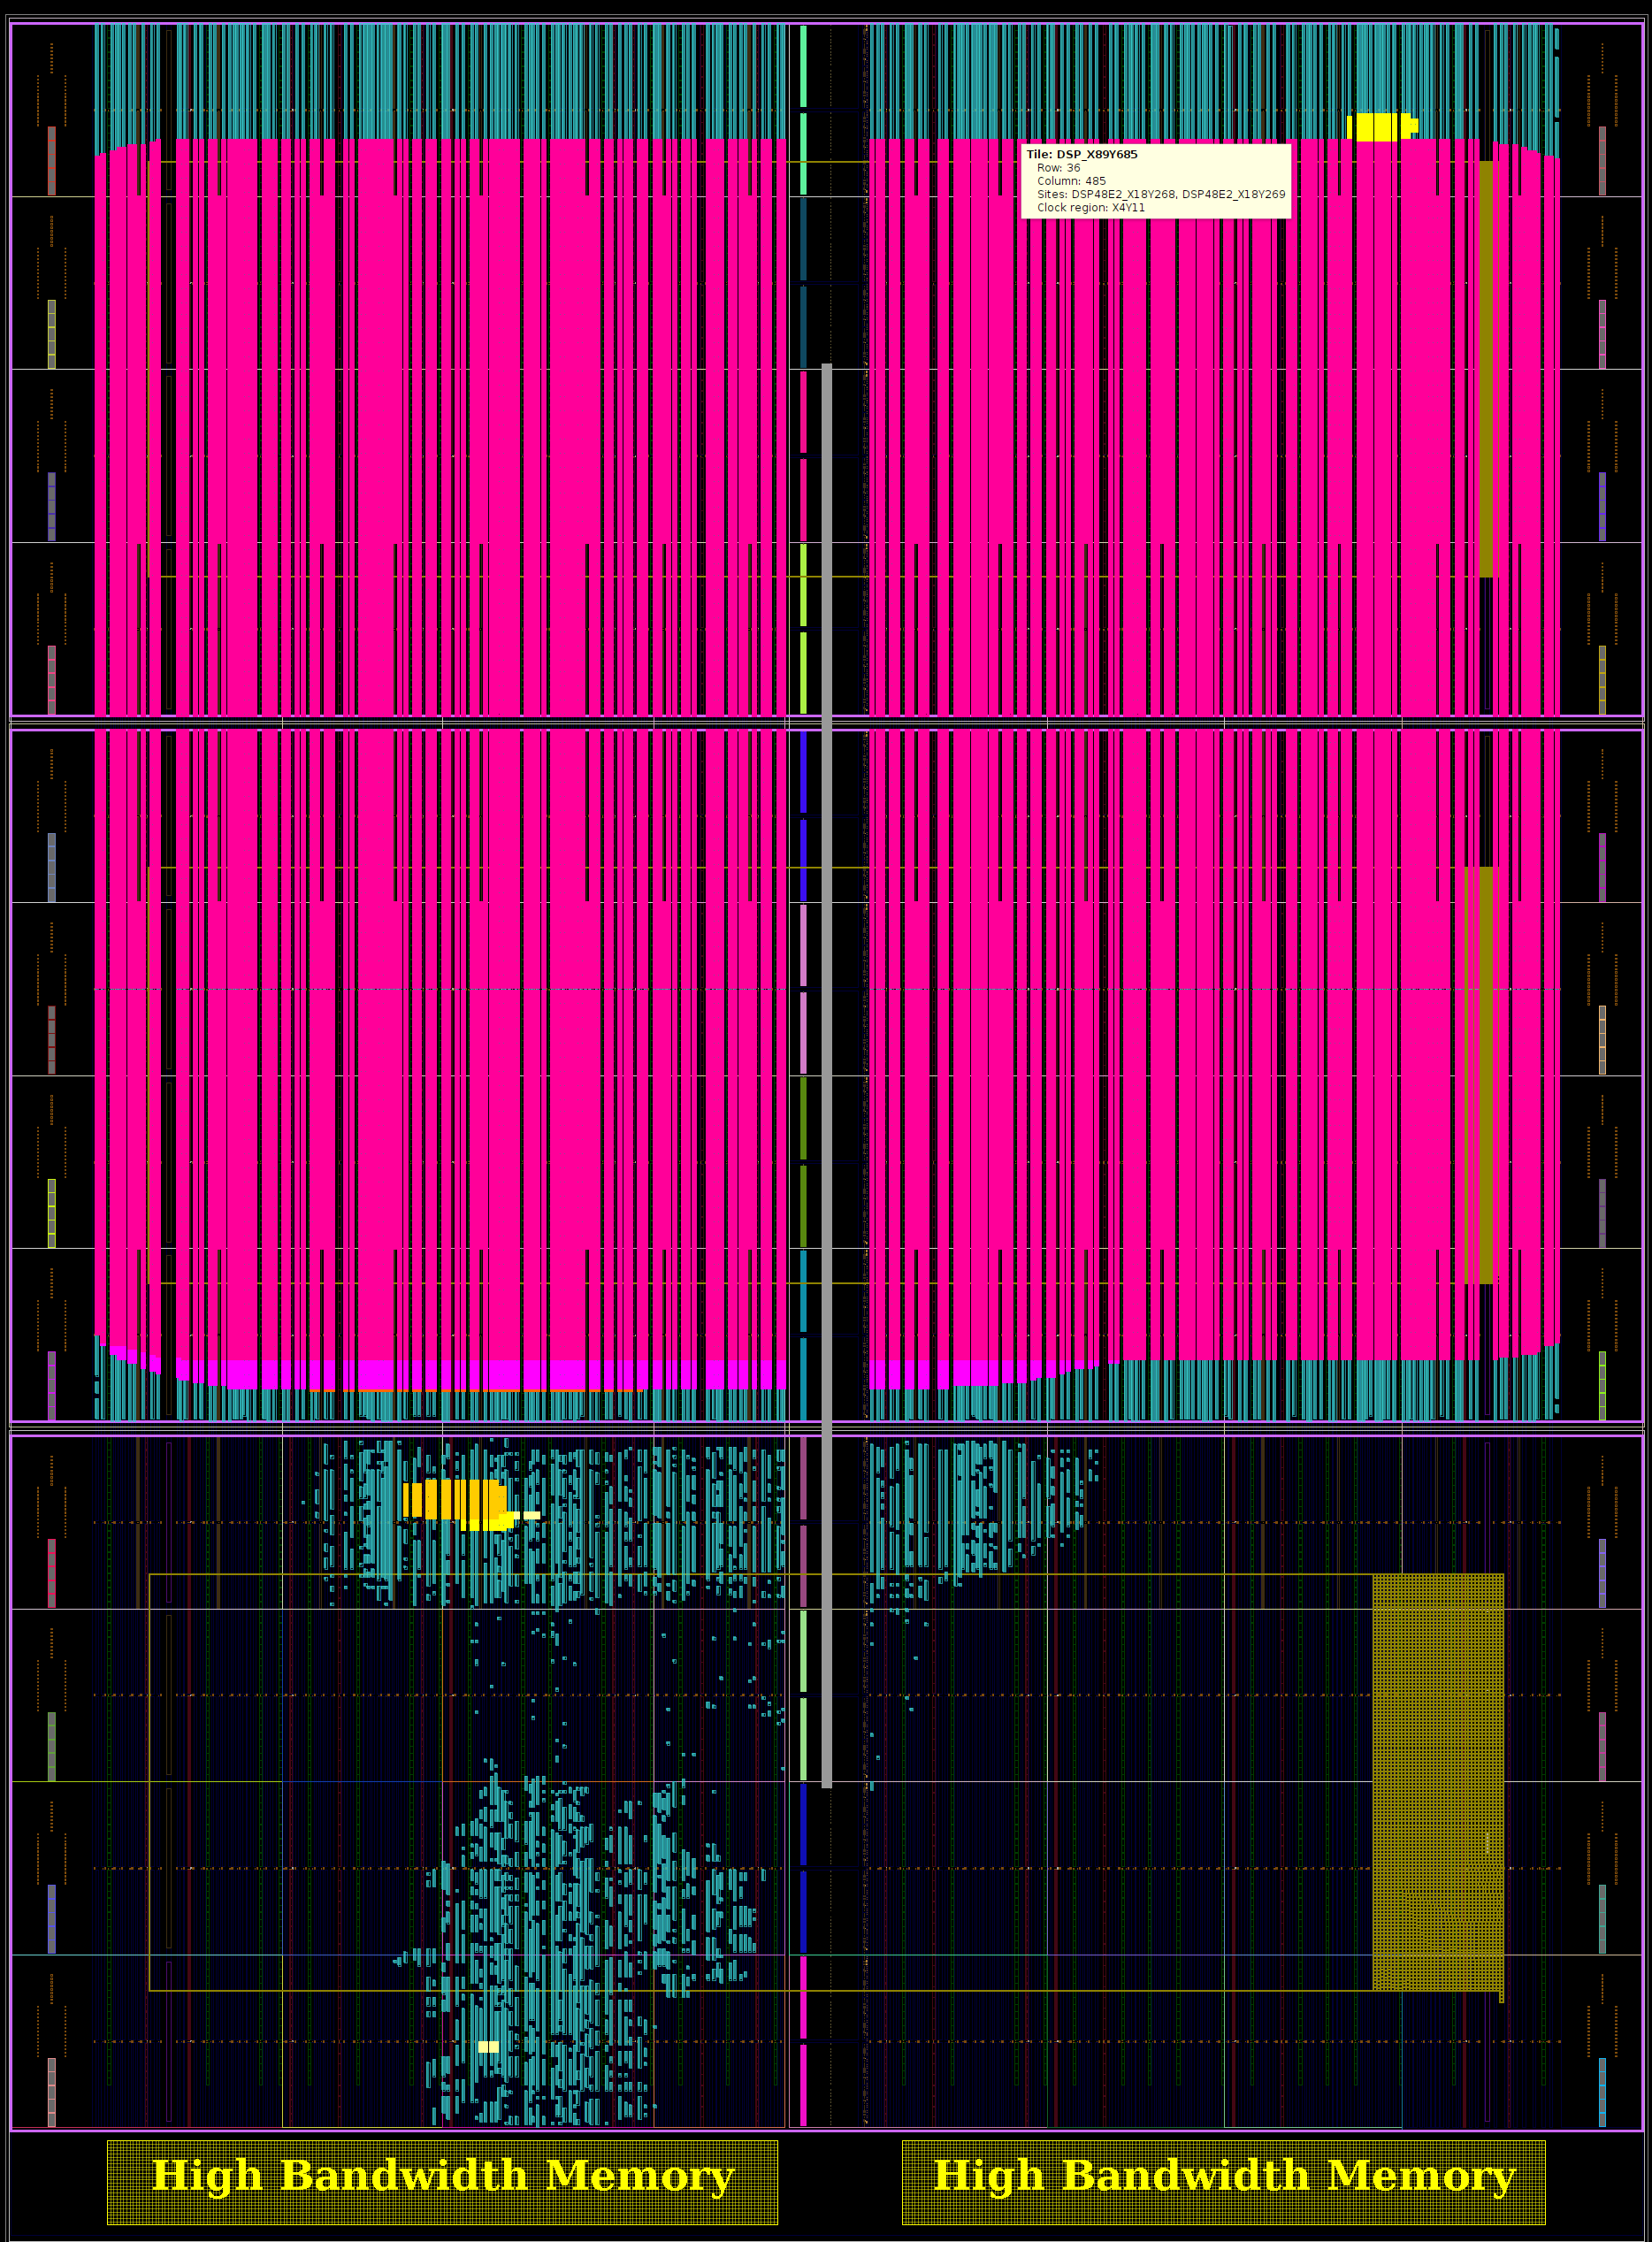
\includegraphics[width=1\columnwidth]{figures/nopblocks}}\hfill{}\subfloat[\texttt{BraggNN} achieves routing closure with use of per SLR placement
and routing constraints (\texttt{pblock\_1}, \texttt{pblock\_2}, \texttt{pblock\_3})
and launch and latch registers (not highlighted).\label{fig:BraggHLS-framework-overview.-2-1-1}]{\centering{}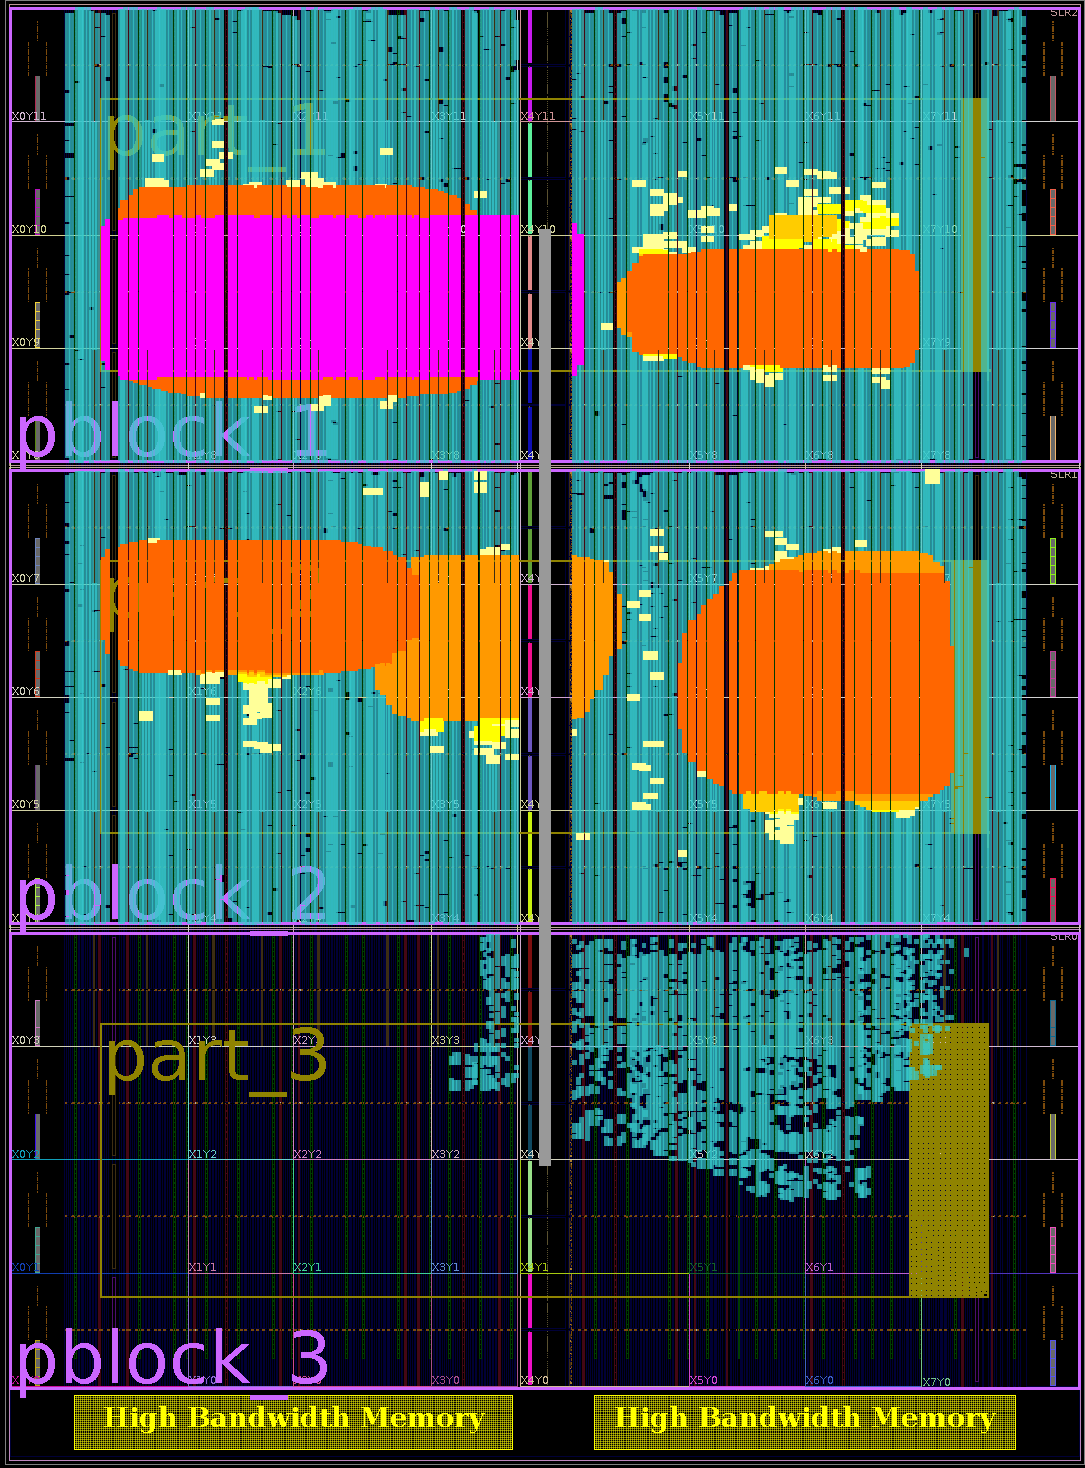
\includegraphics[width=1\columnwidth]{figures/withpblocks}}\caption{Congestion maps for \texttt{BraggNN} on a Xilinx Alveo U280. \textcolor{magenta}{Magenta}
indicates areas of high congestion.\label{fig:BraggHLS-framework-overview.-2}}
\end{figure*}

Thus, the confluence of the aforementioned design choices (in combination
with compiler level optimizations performed by \texttt{BraggHLS})
and careful management of routing constraints enables us to lower,
compile, synthesize, place and route \texttt{BraggNN($s=1$)} to Xilinx's
Alveo U280 at a throughput of 4.8 \textmu s/sample. This is \textasciitilde 5$\times$
higher latency than the target 1 \textmu s/sample but it is a \textasciitilde 4$\times$
improvement over the GPU PyTorch-GPU implementation. In the following
we propose some future work that can further improve on this.

\section{Conclusion\label{sec:Conclusion}}

\printbibliography


\appendix{}

\onecolumn\begin{longtable}{llrrrrrrr}
\caption{Latency, resource usage, and runtimes for all \texttt{BraggHLS} evaluations.}
\label{tab:all_unrolls}\\
\toprule
         & {} & \multicolumn{7}{l}{metric\_val} \\
         & metric\_name &       BRAM &      DSP &       FF &      LUT & Latency & Clock Period &  Runtime \\
module & unroll\_factor &            &          &          &          &         &              &          \\
\midrule
\endfirsthead
\caption[]{Latency, resource usage, and runtimes for all \texttt{BraggHLS} evaluations.} \\
\toprule
         & {} & \multicolumn{7}{l}{metric\_val} \\
         & metric\_name &       BRAM &      DSP &       FF &      LUT & Latency & Clock Period &  Runtime \\
module & unroll\_factor &            &          &          &          &         &              &          \\
\midrule
\endhead
\midrule
\multicolumn{9}{r}{{Continued on next page}} \\
\midrule
\endfoot

\bottomrule
\endlastfoot
addmm & 0    &   0.00E+00 & 2.66E-01 & 3.83E-01 & 2.69E-01 &    1334 &     6.13E+00 & 4.14E+01 \\
         & 4    &   3.97E-01 & 2.66E-01 & 3.90E-01 & 2.94E-01 &    1205 &     6.13E+00 & 4.80E+01 \\
         & 8    &   3.97E-01 & 2.66E-01 & 3.91E-01 & 2.95E-01 &    1205 &     6.13E+00 & 5.73E+01 \\
         & 12   &   3.97E-01 & 8.87E-01 & 1.33E+00 & 8.61E-01 &     993 &     6.14E+00 & 1.16E+02 \\
         & 16   &   3.97E-01 & 8.87E-01 & 1.33E+00 & 8.61E-01 &     993 &     6.14E+00 & 1.19E+02 \\
         & 20   &   3.97E-01 & 1.95E+00 & 1.46E+00 & 1.10E+00 &     900 &     6.14E+00 & 1.30E+02 \\
         & 24   &   3.97E-01 & 3.37E+00 & 1.34E+00 & 1.35E+00 &     888 &     6.14E+00 & 1.79E+02 \\
         & 28   &   3.97E-01 & 2.13E+00 & 1.13E+00 & 1.14E+00 &     821 &     6.46E+00 & 1.14E+02 \\
         & 32   &   3.97E-01 & 2.13E+00 & 1.13E+00 & 1.14E+00 &     821 &     6.46E+00 & 1.15E+02 \\
         & 36   &   3.97E-01 & 2.13E+00 & 1.25E+00 & 1.37E+00 &     425 &     6.43E+00 & 1.63E+02 \\
         & 40   &   3.97E-01 & 2.84E+00 & 1.55E+00 & 2.25E+00 &     359 &     6.42E+00 & 2.55E+02 \\
         & 1024 &   3.97E-01 & 5.67E+00 & 7.86E-01 & 3.74E+00 &     314 &     6.14E+00 & 3.00E+02 \\
batch\_norm & 0    &   0.00E+00 & 1.99E-01 & 4.24E-02 & 1.12E-01 &     116 &     6.06E+00 & 3.36E+01 \\
         & 4    &   0.00E+00 & 1.99E-01 & 4.36E-02 & 1.16E-01 &     116 &     6.06E+00 & 3.16E+01 \\
         & 8    &   0.00E+00 & 2.66E-01 & 2.72E-01 & 2.22E-01 &     125 &     6.06E+00 & 3.57E+01 \\
         & 12   &   0.00E+00 & 1.24E+00 & 3.09E-01 & 6.11E-01 &      69 &     6.06E+00 & 5.05E+01 \\
         & 16   &   0.00E+00 & 1.55E+00 & 1.55E-01 & 5.61E-01 &      23 &     6.06E+00 & 4.90E+01 \\
         & 20   &   0.00E+00 & 1.55E+00 & 1.55E-01 & 5.61E-01 &      23 &     6.06E+00 & 4.94E+01 \\
         & 24   &   0.00E+00 & 1.55E+00 & 1.55E-01 & 5.61E-01 &      23 &     6.06E+00 & 4.92E+01 \\
         & 28   &   0.00E+00 & 1.55E+00 & 1.55E-01 & 5.61E-01 &      23 &     6.06E+00 & 4.98E+01 \\
         & 32   &   0.00E+00 & 1.55E+00 & 1.55E-01 & 5.61E-01 &      23 &     6.06E+00 & 4.86E+01 \\
         & 36   &   0.00E+00 & 1.55E+00 & 1.55E-01 & 5.61E-01 &      23 &     6.06E+00 & 4.85E+01 \\
         & 40   &   0.00E+00 & 1.55E+00 & 1.55E-01 & 5.61E-01 &      23 &     6.06E+00 & 4.98E+01 \\
         & 1024 &   0.00E+00 & 1.55E+00 & 1.55E-01 & 5.61E-01 &      23 &     6.06E+00 & 4.88E+01 \\
braggnn & 0    &   1.51E+00 & 2.22E+00 & 4.34E-01 & 1.09E+00 &   85851 &     7.59E+00 & 1.05E+02 \\
         & 4    &   1.84E+00 & 2.22E+00 & 8.61E-01 & 1.99E+00 &   49310 &     6.45E+00 & 1.38E+02 \\
         & 8    &   1.81E+00 & 2.22E+00 & 8.69E-01 & 2.03E+00 &   49257 &     6.14E+00 & 1.39E+02 \\
         & 12   &   6.70E-01 & 2.22E+00 & 9.56E-01 & 2.25E+00 &   61499 &     6.14E+00 & 2.38E+02 \\
         & 16   &   2.13E+00 & 3.59E+00 & 2.29E+00 & 5.04E+00 &   52515 &     6.40E+00 & 6.52E+02 \\
         & 20   &   2.04E+01 & 1.14E+01 & 2.69E+00 & 7.82E+00 &   51768 &     6.40E+00 & 2.23E+03 \\
         & 24   &   5.21E-01 & 2.01E+01 & 4.95E+00 & 1.22E+01 &   24004 &     6.14E+00 & 7.97E+03 \\
         & 28   &   2.73E-01 & 2.02E+01 & 4.64E+00 & 1.35E+01 &   22377 &     6.42E+00 & 6.85E+03 \\
         & 32   &   2.98E-01 & 7.01E+01 & 1.07E+01 & 3.29E+01 &    9793 &     6.42E+00 & 1.01E+04 \\
         & 36   &   2.98E-01 & 6.73E+01 & 1.15E+01 & 4.27E+01 &    9730 &     6.42E+00 & 1.23E+04 \\
         & 40   &   2.98E-01 & 8.21E+01 & 1.40E+01 & 7.83E+01 &    9032 &     6.42E+00 & 6.18E+04 \\
         & 1024 &   3.22E-01 & 3.46E+01 & 8.27E+00 & 9.48E+01 &    6789 &     6.14E+00 & 4.67E+04 \\
conv & 0    &   0.00E+00 & 4.43E-02 & 2.30E-02 & 4.40E-02 &    3551 &     6.13E+00 & 2.69E+01 \\
         & 4    &   0.00E+00 & 4.43E-02 & 2.30E-02 & 4.40E-02 &    3551 &     6.13E+00 & 2.64E+01 \\
         & 8    &   0.00E+00 & 4.43E-02 & 2.30E-02 & 4.40E-02 &    3551 &     6.13E+00 & 2.66E+01 \\
         & 12   &   0.00E+00 & 3.77E-01 & 7.04E-01 & 1.97E+00 &    1310 &     6.14E+00 & 1.33E+03 \\
         & 16   &   0.00E+00 & 3.77E-01 & 7.03E-01 & 1.98E+00 &    1310 &     6.14E+00 & 1.32E+03 \\
         & 20   &   0.00E+00 & 3.77E-01 & 7.03E-01 & 1.98E+00 &    1310 &     6.14E+00 & 1.34E+03 \\
         & 24   &   0.00E+00 & 3.77E-01 & 7.03E-01 & 1.97E+00 &    1310 &     6.14E+00 & 1.35E+03 \\
         & 28   &   0.00E+00 & 3.77E-01 & 7.03E-01 & 1.97E+00 &    1310 &     6.14E+00 & 1.33E+03 \\
         & 32   &   0.00E+00 & 3.77E-01 & 7.03E-01 & 1.97E+00 &    1310 &     6.14E+00 & 1.37E+03 \\
         & 36   &   0.00E+00 & 3.77E-01 & 7.03E-01 & 1.97E+00 &    1310 &     6.14E+00 & 1.38E+03 \\
         & 40   &   0.00E+00 & 1.97E+00 & 6.49E-01 & 5.07E+00 &     795 &     6.14E+00 & 2.05E+02 \\
         & 1024 &   0.00E+00 & 1.97E+00 & 6.49E-01 & 5.07E+00 &     795 &     6.14E+00 & 2.09E+02 \\
max\_pool\_2d & 0    &   0.00E+00 & 0.00E+00 & 4.41E-03 & 2.72E-02 &     889 &     3.28E+00 & 3.11E+01 \\
         & 4    &   0.00E+00 & 0.00E+00 & 4.41E-03 & 2.72E-02 &     889 &     3.28E+00 & 3.05E+01 \\
         & 8    &   0.00E+00 & 0.00E+00 & 2.40E-02 & 8.04E-02 &     641 &     6.20E+00 & 3.63E+01 \\
         & 12   &   0.00E+00 & 0.00E+00 & 2.40E-02 & 8.04E-02 &     641 &     6.20E+00 & 3.66E+01 \\
         & 16   &   0.00E+00 & 0.00E+00 & 1.10E+00 & 7.63E-01 &     419 &     2.32E+01 & 9.40E+01 \\
         & 20   &   0.00E+00 & 0.00E+00 & 1.04E+00 & 7.51E-01 &     412 &     2.39E+01 & 9.56E+01 \\
         & 24   &   0.00E+00 & 0.00E+00 & 2.25E-01 & 1.03E+00 &     262 &     3.81E+01 & 6.22E+01 \\
         & 28   &   0.00E+00 & 0.00E+00 & 2.25E-01 & 1.03E+00 &     262 &     3.81E+01 & 6.34E+01 \\
         & 32   &   0.00E+00 & 0.00E+00 & 2.25E-01 & 1.03E+00 &     262 &     3.81E+01 & 6.29E+01 \\
         & 36   &   0.00E+00 & 0.00E+00 & 2.25E-01 & 1.03E+00 &     262 &     3.81E+01 & 6.30E+01 \\
         & 40   &   0.00E+00 & 0.00E+00 & 2.25E-01 & 1.03E+00 &     262 &     3.81E+01 & 6.25E+01 \\
         & 1024 &   0.00E+00 & 0.00E+00 & 2.25E-01 & 1.03E+00 &     262 &     3.81E+01 & 6.24E+01 \\
soft\_max & 0    &   2.23E-01 & 4.43E-02 & 3.49E-02 & 9.52E-02 &    7742 &     6.38E+00 & 3.99E+01 \\
         & 4    &   2.23E-01 & 8.87E-02 & 6.01E-02 & 1.27E-01 &    5053 &     6.13E+00 & 3.83E+01 \\
         & 8    &   2.23E-01 & 8.87E-02 & 6.50E-02 & 1.44E-01 &    5053 &     6.13E+00 & 4.31E+01 \\
         & 12   &   0.00E+00 & 7.09E-01 & 2.53E-01 & 9.04E-01 &    3037 &     6.13E+00 & 6.06E+01 \\
         & 16   &   0.00E+00 & 7.09E-01 & 2.53E-01 & 9.04E-01 &    3037 &     6.13E+00 & 5.90E+01 \\
         & 20   &   2.78E+00 & 1.42E+00 & 5.82E-01 & 1.16E+00 &    2893 &     6.14E+00 & 1.54E+02 \\
         & 24   &   2.78E+00 & 1.42E+00 & 7.64E-01 & 1.39E+00 &    2893 &     6.14E+00 & 4.15E+02 \\
         & 28   &   0.00E+00 & 1.70E+01 & 7.17E+00 & 1.07E+01 &    2277 &     6.14E+00 & 9.14E+02 \\
         & 32   &   0.00E+00 & 1.70E+01 & 7.17E+00 & 1.07E+01 &    2277 &     6.14E+00 & 9.16E+02 \\
         & 36   &   0.00E+00 & 1.72E+01 & 1.97E+00 & 4.45E+00 &    1684 &     6.14E+00 & 4.66E+02 \\
         & 40   &   0.00E+00 & 1.72E+01 & 1.97E+00 & 4.45E+00 &    1684 &     6.14E+00 & 4.60E+02 \\
         & 1024 &   0.00E+00 & 1.72E+01 & 1.97E+00 & 4.45E+00 &    1684 &     6.14E+00 & 4.63E+02 \\
\end{longtable}
\twocolumn
\begin{table*}[tbh]
\caption{Resource usage for \texttt{BraggNN($s=1$)} and $\left(5,3\right)$-precision
FloPoCo \label{tab:Resource-usage-for}}

\begin{centering}
\begin{tabular}{lllllll}
\toprule
Site Type & SLR0 & SLR1 & SLR2 & SLR0 \% & SLR1 \% & SLR2 \%\tabularnewline
\midrule
CLB & 5047 & 52648 & 53900 & 9.18 & 97.50 & 99.81\tabularnewline
\midrule
\quad{}CLBL & 2773 & 28613 & 29227 & 9.47 & 97.72 & 99.82\tabularnewline
\midrule
\quad{}CLBM & 2274 & 24035 & 24673 & 8.86 & 97.23 & 99.81\tabularnewline
\midrule
CLB LUTs & 19797 & 263733 & 311794 & 4.50 & 61.05 & 72.17\tabularnewline
\midrule
\quad{}LUT as Logic & 19797 & 263733 & 311794 & 4.50 & 61.05 & 72.17\tabularnewline
\midrule
\quad{}\quad{}using O5 output only & 277 & 3944 & 4304 & 0.06 & 0.91 & 1.00\tabularnewline
\midrule
\quad{}\quad{}using O6 output only & 17176 & 202564 & 266733 & 3.91 & 46.89 & 61.74\tabularnewline
\midrule
\quad{}\quad{}using O5 and O6 & 2344 & 57225 & 40757 & 0.53 & 13.25 & 9.43\tabularnewline
\midrule
\quad{}LUT as Memory & 0 & 0 & 0 & 0.00 & 0.00 & 0.00\tabularnewline
\midrule
\quad{}\quad{}LUT as Distributed RAM & 0 & 0 & 0 & 0.00 & 0.00 & 0.00\tabularnewline
\midrule
\quad{}\quad{}LUT as Shift Register & 0 & 0 & 0 & 0.00 & 0.00 & 0.00\tabularnewline
\midrule
CLB Registers & 12527 & 286226 & 339820 & 1.42 & 33.13 & 39.33\tabularnewline
\midrule
CARRY8 & 244 & 5184 & 5184 & 0.44 & 9.60 & 9.60\tabularnewline
\midrule
Block RAM Tile & 0 & 0 & 0 & 0.00 & 0.00 & 0.00\tabularnewline
\midrule
\quad{}\quad{}RAMB36/FIFO & 0 & 0 & 0 & 0.00 & 0.00 & 0.00\tabularnewline
\midrule
\quad{}\quad{}RAMB18 & 0 & 0 & 0 & 0.00 & 0.00 & 0.00\tabularnewline
\midrule
URAM & 0 & 0 & 0 & 0.00 & 0.00 & 0.00\tabularnewline
\midrule
DSPs & 0 & 0 & 0 & 0.00 & 0.00 & 0.00\tabularnewline
\midrule
Unique Control Sets & 189 & 2641 & 3179 & 0.17 & 2.45 & 2.94\tabularnewline
\bottomrule
\end{tabular}
\par\end{centering}
\bigskip{}

\begin{centering}
\caption{Super long line usage across super logic regions for \texttt{BraggNN}\label{tab:Resource-usage-for-1}}
\par\end{centering}
\centering{}%
\begin{tabular}{lllll}
\toprule
~ & Used & Fixed & Available & Util \%\tabularnewline
\midrule
SLR2 $\leftrightarrow$ SLR1 & 21366 & ~ & 23040 & 92.73\tabularnewline
\midrule
SLR1 $\rightarrow$ SLR2 & 2 & ~ & ~ & < 0.01\tabularnewline
\midrule
SLR2 $\rightarrow$ SLR1 & 21364 & ~ & ~ & 92.73\tabularnewline
\midrule
SLR1 $\leftrightarrow$ SLR0 & 3904 & ~ & 23040 & 16.94\tabularnewline
\midrule
SLR0 $\rightarrow$ SLR1 & 2 & ~ & ~ & < 0.01\tabularnewline
\midrule
SLR1 $\rightarrow$ SLR0 & 3902 & ~ & ~ & 16.94\tabularnewline
\midrule
Total SLLs Used & 25270 & ~ & ~ & ~\tabularnewline
\bottomrule
\end{tabular}
\end{table*}

\end{document}
